\documentclass[12pt]{article}
\usepackage{OSUDissertation}

\begin{document}

\setlength{\abovedisplayskip}{5pt}
\setlength{\belowdisplayskip}{5pt}

%%%%%%%%%%%%%%%%%%%%%%%%%%%%%%%%%%%%%%%
\section{\RZ\ Geometry}
\label{sec:RZ}
Solving the transport equation in different coordinate systems may provide simpler ways of modeling a particular geometry or symmetry. In this section, we derive the \RZ\ transport equation to be solved. It assumes there is no variation in the azimuthal direction (of a cylinder), hence problems in \RZ\ geometry look very similar to problems in \XY\ geometry. The streaming operator in cylindrical geometry is \cite{Lewis_Comp_Methods_Neu_Trans}
\begin{flalign}
\vec{\Omega} \vd \grad \psi & = \frac{\mu}{r} \frac{\partial}{\partial r} (r \psi) + \frac{\eta}{r} \frac{\partial \psi}{\partial \zeta} + \xi \frac{\partial \psi}{\partial z} - \frac{1}{r} \frac{\partial}{\partial \omega} (\eta \psi),
\end{flalign}
%
where $\vec{\Omega}$ is the direction of travel unit vector, $\psi$ is the angular flux, and
\begin{flalign}
\mu & \equiv \vec{\Omega} \vd \hat{e}_r = \sqrt{1 - \xi^2} \cos \omega = \sin(\theta) \cos(\omega), \\
\eta & \equiv \vec{\Omega} \vd \hat{e}_\theta = \sqrt{1 - \xi^2} \sin \omega = \sin(\theta) \sin(\omega), \\
\xi & \equiv \vec{\Omega} \vd \hat{e}_z = \cos(\theta).
\end{flalign}
%
The variables $\mu$, $\eta$, $\xi$, $\omega$, and $\theta$ are shown in the cylindrical coordinate system in Figure \ref{fig:CylindricalCoordinateSystem}. We assume there is no solution variation in the azimuthal direction, i.e.
\begin{flalign}
\frac{\partial \psi}{\partial \zeta} & \equiv 0,
\end{flalign}
%
which simplifies the streaming term to
\begin{flalign}
\vec{\Omega} \vd \grad \psi & = \frac{\mu}{r} \frac{\partial}{\partial r} (r \psi) + \xi \frac{\partial \psi}{\partial z} - \frac{1}{r} \frac{\partial}{\partial \omega} (\eta \psi).
\end{flalign}

\begin{figure}[!h]
\tdplotsetmaincoords{60}{110}
\begin{tikzpicture}[scale=10,tdplot_main_coords]
\pgfmathsetmacro{\rvec}{.8}
\pgfmathsetmacro{\phivec}{40}
\pgfmathsetmacro{\thetavec}{50}
\pgfmathsetmacro{\omegavec}{60}

\coordinate (O) at (0,0,0);
\draw[thick,->] (0,0,0) -- (1,0,0) node[anchor=north east]{$x$};
\draw[thick,->] (0,0,0) -- (0,1,0) node[anchor=north west]{$y$};
\draw[thick,->] (0,0,0) -- (0,0,1) node[anchor=south]{$z$};
\tdplotsetcoord{P}{\rvec}{\phivec}{\thetavec}
\draw[-stealth,color=red] (O) -- (P) node[above left] {$(r,z)$};
\draw[dashed, color=red] (O) -- (Pxy);
\draw[dashed, color=red] (P) -- (Pxy);
\tdplotdrawarc[color=red,->]{(O)}{0.2}{0}{\thetavec}{anchor=north}{$\zeta$}

\coordinate (er) at ($(P)+0.4*({cos(\thetavec)},{sin(\thetavec)},0)$);
\coordinate (etheta) at ($(P)+0.4*({-cos(90-\thetavec)},{sin(90-\thetavec)},0)$);
\coordinate (ez) at ($(P)+0.4*(0,0,1)$);
\draw[-stealth] (P) -- (er) node[below right] {$\hat{e}_r$};
\draw[-stealth] (P) -- (etheta) node[below right] {$\hat{e}_\theta$};
\draw[-stealth] (P) -- (ez) node[right] {$\hat{e}_z$};

\coordinate (Omega) at ($(P)+0.2*(-.5,1.5,2)$);
\draw[-stealth,color=blue] (P) -- (Omega) node[above right] {$\vec{\Omega}$};
\draw[dashed,color=blue] (Omega) -- ($(Omega)+0.2*(0,0,-2)$) -- (P);
\tdplotdrawarc[color=blue,->]{(P)}{0.2}{\thetavec}{\thetavec+\omegavec}{anchor=north}{$\omega$}

\tdplotsetthetaplanecoords{\phivec}
\tdplotsetrotatedcoords{\thetavec}{270}{0}
\tdplotsetrotatedcoordsorigin{(P)}
\tdplotdrawarc[tdplot_rotated_coords,color=blue,->]{(0,0,0)}{0.2}{0}{\thetavec}{anchor=south west}{$\theta$}

\end{tikzpicture}
\caption{Cylindrical space-angle coordinate system showing the position $(r,z)$ and direction of travel $\vec{\Omega}$.}
\label{fig:CylindricalCoordinateSystem}
\end{figure}

The transport equation in \RZ\ geometry is then
\begin{multline}
\frac{\mu}{r} \frac{\partial}{\partial r} r \psi \left(r,z, \vec{\Omega} \right) + \xi \frac{\partial}{\partial z} \psi \left(r,z,\vec{\Omega} \right) - \frac{1}{r} \frac{\partial}{\partial \omega} \eta \psi \left(r,z, \vec{\Omega} \right) + \sigma_t \left(r,z \right) \psi \left(r,z,\vec{\Omega} \right) \\
= \frac{1}{4 \pi} \int_{4 \pi} \sigma_s \left(r,z \right) I \left(r,z, \vec{\Omega}^\prime \right) d \Omega^\prime + S_0 \left(r,z, \vec{\Omega} \right)
\label{eq:RZTransport}
\end{multline}

\noindent where $\sigma_t$ is the total cross section, $\sigma_s$ is the scattering cross section, and $S_0$ is an isotropic source as before. The streaming term describes the motion of the particle density into or out of a volume. Since the streaming term now has an angular derivative (two angular derivatives in 3-D), the spatial streaming now depends on the direction of travel. The $\hat{e}_r$ axis in Figure~\ref{fig:CylindricalCoordinateSystem} is always in the same direction as the $r$-axis. Considering a particle traveling in a straight direction $\vec{\Omega}$, as the particle changes position, the coordinate axis defining $\vec{\Omega}$ changes. This couples the spatial and angular axes when defining the phase space of a particle. First, we must discretize the direction of particle travel.

%%%%%%%%%%%%%%%%%%%%%%%%%%%%%%%%%%%%%%%
\subsection{Angular Discretization}
Discretizing Equation \ref{eq:RZTransport} with a level-symmetric angular quadrature results in 
\begin{multline}
\frac{\mu_{n,m}}{r} \frac{\partial}{\partial r} r \psi_{n,m} \left(r,z \right) + \xi_n \frac{\partial}{\partial z} \psi_{n,m} \left(r,z \right) - \frac{1}{r} \frac{\partial}{\partial \omega} \eta_{n,m} \psi_{n,m} \left(r,z \right) + \sigma_t \left(r,z \right) \psi_{n,m} \left(r,z \right) \\
= \frac{1}{4 \pi} \int_{4 \pi} \sigma_s \left(r,z \right) I \left(r,z, \vec{\Omega}^\prime \right) d \Omega^\prime + S_0 \left(r,z, \vec{\Omega} \right)
\label{eq:RZSNTransport}
\end{multline}

\noindent for direction $\vec{\Omega}_{n,m}$, where index $n$ describes a level of quadrature with constant $\xi$ and the $m$ index denotes the quadrature point on that level. The $(n,m)$ indexing is shown in Figure \ref{fig:AngularDiscretization}.

\begin{figure}[!htb]
\centering
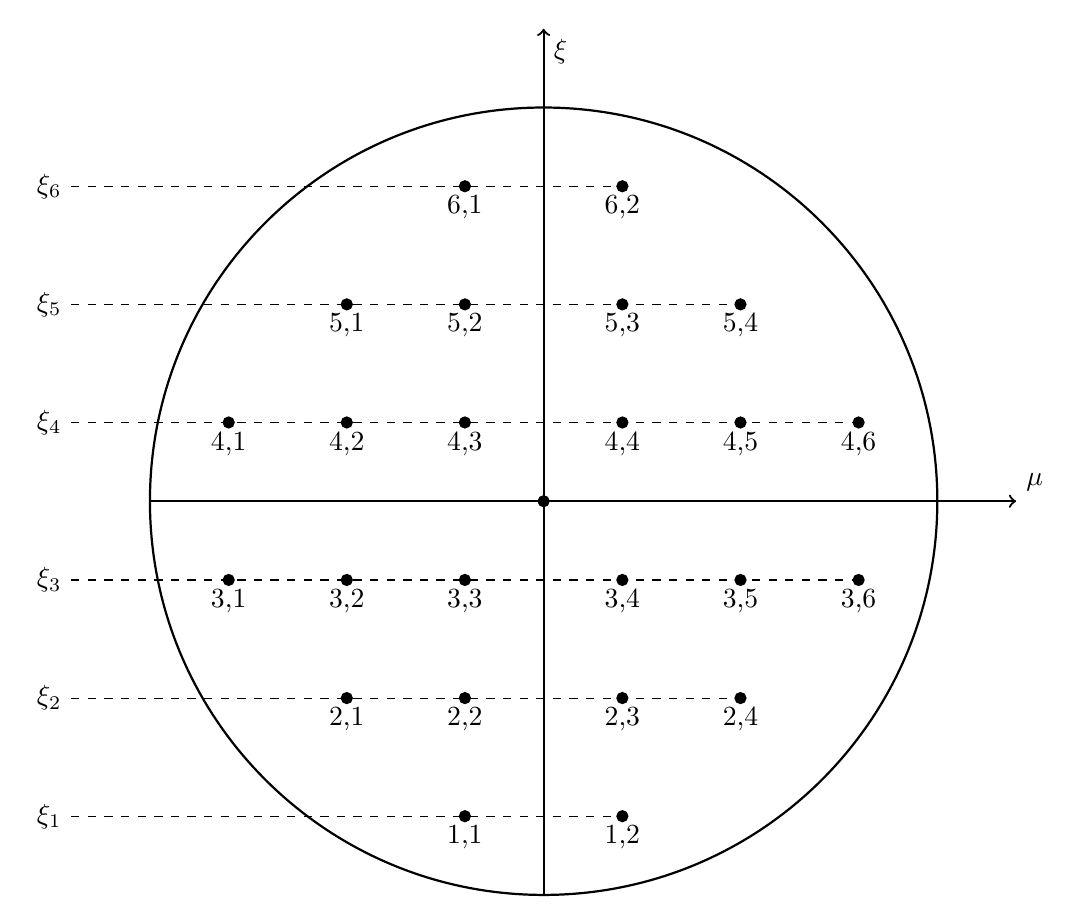
\begin{tikzpicture}

\draw[fill=black] (0,0) circle (2pt);
\draw[thick,->] (-5,0) -- (6,0) node[above right]{$\mu$};
\draw[thick,->] (0,-5) -- (0,6) node[below right]{$\xi$};
\draw[thick] (0,0) circle (5cm);

\draw[dashed] (-6,-4) node[left]{$\xi_1$} -- (1,-4);
\draw[dashed] (-6,-2.5) node[left]{$\xi_2$} -- (2.5,-2.5);
\draw[dashed] (-6,-1) node[left]{$\xi_3$} -- (4,-1);
\draw[dashed] (-6,1) node[left]{$\xi_4$} -- (4,1);
\draw[dashed] (-6,2.5) node[left]{$\xi_5$} -- (2.5,2.5);
\draw[dashed] (-6,4) node[left]{$\xi_6$} -- (1,4);

\draw[fill=black] (-4,-1) circle (2pt) node[below]{3,1};
\draw[fill=black] (-2.5,-1) circle (2pt) node[below]{3,2};
\draw[fill=black] (-1,-1) circle (2pt) node[below]{3,3};
\draw[fill=black] (-2.5,-2.5) circle (2pt) node[below]{2,1};
\draw[fill=black] (-1, -2.5) circle (2pt) node[below]{2,2};
\draw[fill=black] (-1,-4) circle (2pt) node[below]{1,1};

\draw[fill=black] (1,-1) circle (2pt) node[below]{3,4};
\draw[fill=black] (2.5,-1) circle (2pt) node[below]{3,5};
\draw[fill=black] (4,-1) circle (2pt) node[below]{3,6};
\draw[fill=black] (1, -2.5) circle (2pt) node[below]{2,3};
\draw[fill=black] (2.5,-2.5) circle (2pt) node[below]{2,4};
\draw[fill=black] (1,-4) circle (2pt) node[below]{1,2};

\draw[fill=black] (-4,1) circle (2pt) node[below]{4,1};
\draw[fill=black] (-2.5,1) circle (2pt) node[below]{4,2};
\draw[fill=black] (-1,1) circle (2pt) node[below]{4,3};
\draw[fill=black] (-2.5,2.5) circle (2pt) node[below]{5,1};
\draw[fill=black] (-1, 2.5) circle (2pt) node[below]{5,2};
\draw[fill=black] (-1,4) circle (2pt) node[below]{6,1};

\draw[fill=black] (1,1) circle (2pt) node[below]{4,4};
\draw[fill=black] (2.5,1) circle (2pt) node[below]{4,5};
\draw[fill=black] (4,1) circle (2pt) node[below]{4,6};
\draw[fill=black] (1, 2.5) circle (2pt) node[below]{5,3};
\draw[fill=black] (2.5,2.5) circle (2pt) node[below]{5,4};
\draw[fill=black] (1,4) circle (2pt) node[below]{6,2};

\end{tikzpicture}
\caption{Angular discretization showing $(\xi,\mu)$ pairs; adapted from \cite{Lewis_Comp_Methods_Neu_Trans}}
\label{fig:AngularDiscretization}
\end{figure}

One of the major challenges is handling the anglar derivative term. Lewis and Miller \cite{Lewis_Comp_Methods_Neu_Trans} describes an approximation for the partial derivative of the intensity with respect to $\omega$:
\begin{flalign}
- \frac{1}{r} \frac{\partial}{\partial \omega} \eta_{m,n} \psi_{n,m} \left(r,z \right) & = \frac{\alpha_{m+1/2}^n \psi_{n,m+1/2} (r,z) - \alpha_{m-1/2}^n \psi_{n,m-1/2} (r,z)}{r w_{n,m}}
\end{flalign}

\noindent where $\alpha_{m+1/2}^n$ and $\alpha_{m-1/2}^n$ are angular differencing coefficients, and $w_{n,m}$ is the angular quadrature weight. We substitute this into Equation \ref{eq:RZSNTransport},
\begin{multline}
\frac{\mu_{n,m}}{r} \frac{\partial}{\partial r} r \psi_{n,m} \left(r,z \right) + \xi_n \frac{\partial}{\partial z} \psi_{n,m} \left(r,z \right) \\
+ \frac{\alpha_{m+1/2}^n \psi_{m+1/2,n} (r,z) - \alpha_{m-1/2}^n \psi_{m-1/2,n} (r,z)}{r w_{n,m}} + \sigma_t \left(r,z \right) \psi_{n,m} \left(r,z \right) \\
= \frac{1}{4 \pi} \int_{4 \pi} \sigma_s \left(r,z \right) \psi \left(r,z, \vec{\Omega}^\prime \right) d \Omega^\prime + \frac{1}{4 \pi} S_0 \left(r,z \right)
\label{eq:RZSNADTransport}
\end{multline}

\noindent Here, we pause to notice that there are similarities and differences between our Cartesian discretization. The absorption term, axial derivative term, and right-hand-side are the same in both coordinate systems. The differences arise in the radial and angular derivative terms. 


After multiplying through by the radius $r$, the radial derivative term has a factor of $r$ inside the derivative. The angular derivative term is also new and does not resemble a mass matrix so MFEM will require additional modification.

Requiring Equation \ref{eq:RZSNADTransport} to satisfy the uniform infinite medium solution results in the condition,
\begin{flalign}
\alpha_{m+1/2}^n & = \alpha_{m-1/2}^n - \mu_{n,m} w_{n,m}
\label{eq:AlphaMinusMuW}
\end{flalign}

\iffalse
\begin{multline}
\int_{4 \pi} d \Omega \left[ \frac{\mu_{n,m}}{r} \frac{\partial}{\partial r} r \psi_{n,m} \left(r,z \right) + \frac{\alpha_{m+1/2}^n \psi_{m+1/2,n} (r,z) - \alpha_{m-1/2}^n \psi_{m-1/2,n} (r,z)}{r w_{n,m}} \right. \\
\left. + \xi_n \frac{\partial}{\partial z} \psi_{n,m} \left(r,z \right) \right] + \sigma_t \left(r,z \right) \phi \left(r,z \right) \\
= \sigma_s \left(r,z \right) \phi \left(r,z\right) + S_0 \left(r,z \right)
\end{multline}
\begin{multline}
\int_{4 \pi} d \Omega \left[ \frac{\mu_{n,m}}{r} \frac{\partial}{\partial r} r \psi_{n,m} \left(r,z \right) + \frac{\alpha_{m+1/2}^n \psi_{m+1/2,n} (r,z) - \alpha_{m-1/2}^n \psi_{m-1/2,n} (r,z)}{r w_{n,m}} \right. \\
\left. + \xi_n \frac{\partial}{\partial z} \psi_{n,m} \left(r,z \right) \right] = 0
\end{multline}

\noindent That is, the streaming term must equal zero because $\sigma_t = \sigma_a + \sigma_s$. Using the product rule,
\begin{multline}
\int_{4 \pi} d \Omega \left[\frac{\mu_{n,m}}{r} \left(\frac{\partial r}{\partial r} \psi_{n,m} + r \frac{\partial \psi_{n,m} (r,z)}{\partial r} \right) + \right. \\
\left. \frac{\alpha_{m+1/2}^n \psi_{m+1/2,n} (r,z) - \alpha_{m-1/2}^n \psi_{m-1/2,n} (r,z)}{r w_{n,m}} + \xi_n \frac{\partial}{\partial z} \psi_{n,m} \left(r,z \right) \right] = 0
\end{multline}
\begin{flalign}
\int_{4 \pi} d \Omega \left[\frac{\mu_{n,m}}{r} \psi_{n,m} + \frac{\alpha_{m+1/2}^n \psi_{m+1/2,n} (r,z) - \alpha_{m-1/2}^n \psi_{m-1/2,n} (r,z)}{r w_{n,m}} \right] & = 0 \\
\left(\frac{\mu_{n,m}}{r} + \frac{\alpha_{m+1/2}^n - \alpha_{m-1/2}^n}{r w_{n,m}} \right) \phi(r,z) & = 0
\end{flalign}

\noindent results in the condition,
\begin{flalign}
\alpha_{m+1/2}^n & = \alpha_{m-1/2}^n - \mu_{n,m} w_{n,m}
\label{eq:AlphaMinusMuW}
\end{flalign}
\fi

\noindent If $\alpha_{1/2}^n$ is known, then the remaining coefficients are uniquely determined. To find $\alpha_{1/2}^n$, we require that Equation \ref{eq:RZSNADTransport} satisfy the conservation equation (Eq. \ref{eq:RZTransport}).
%
\iffalse
Discretizing Equation \ref{eq:RZTransport} using discrete ordinates and summing over all directions (approximately integrating over all directions),
\begin{multline}
\sum_{n=1}^N \sum_{m=1}^{M_n} \frac{1}{r} \frac{\partial}{\partial r} r w_{n,m} \mu_{n,m} \psi_{n,m} \left(r,z \right) - \sum_{n=1}^N \sum_{m=1}^{M_n} \frac{1}{r} \frac{\partial}{\partial \omega} w_{n,m} \eta_{n,m} \psi_{n,m} \left(r,z \right) \\
+ \sum_{n=1}^N \sum_{m=1}^{M_n} \xi_n \frac{\partial}{\partial z} w_{n,m} \psi_{n,m} \left(r,z \right) + \sum_{n=1}^N \sum_{m=1}^{M_n} \sigma_t \left(r,z \right) \psi_{n,m} \left(r,z \right) \\
= \sum_{n=1}^N \sum_{m=1}^{M_n} w_{n,m} \frac{1}{4 \pi} \int_{4 \pi} \sigma_s \left(r,z \right) \psi \left(r,z, \vec{\Omega}^\prime \right) d \Omega^\prime + \sum_{n=1}^N \sum_{m=1}^{M_n} w_{n,m} \frac{1}{4 \pi} S_0 \left(r,z \right)
\end{multline}

\noindent Given that the sum of the weights is $\sum w = 4 \pi$,
\begin{multline}
\sum_{n=1}^N \sum_{m=1}^{M_n} \frac{1}{r} \frac{\partial}{\partial r} r w_{n,m} \mu_{n,m} \psi_{n,m} \left(r,z \right) - \sum_{n=1}^N \sum_{m=1}^{M_n} \frac{1}{r} \frac{\partial}{\partial \omega} w_{n,m} \eta_{n,m} \psi_{n,m} \left(r,z \right) \\
+ \sum_{n=1}^N \sum_{m=1}^{M_n} \xi_n \frac{\partial}{\partial z} w_{n,m} \psi_{n,m} \left(r,z \right) \\
= - \sum_{n=1}^N \sum_{m=1}^{M_n} \sigma_t \left(r,z \right) \psi_{n,m} \left(r,z \right) + \int_{4 \pi} \sigma_s \left(r,z \right) \psi \left(r,z, \vec{\Omega}^\prime \right) d \Omega^\prime +  S_0 \left(r,z \right)
\end{multline}

\noindent Multiplying Equation \ref{eq:RZSNADTransport} by weight $w_{n,m}$ and summing over all directions results in
\begin{multline}
\sum_{n=1}^N \sum_{m=1}^{M_n} w_{n,m} \frac{\mu_{n,m}}{r} \frac{\partial}{\partial r} r \psi_{n,m} \left(r,z \right) + \sum_{n=1}^N \sum_{m=1}^{M_n} w_{n,m} \frac{\alpha_{m+1/2}^n \psi_{m+1/2,n} (r,z) - \alpha_{m-1/2}^n \psi_{m-1/2,n} (r,z)}{r w_{n,m}} \\
+ \sum_{n=1}^N \sum_{m=1}^{M_n} w_{n,m} \xi_n \frac{\partial}{\partial z} \psi_{n,m} \left(r,z \right) + \sum_{n=1}^N \sum_{m=1}^{M_n} w_{n,m} \sigma_t \left(r,z \right) \psi_{n,m} \left(r,z \right) \\
= \sum_{n=1}^N \sum_{m=1}^{M_n} w_{n,m} \frac{1}{4 \pi} \int_{4 \pi} \sigma_s \left(r,z \right) \psi \left(r,z, \vec{\Omega}^\prime \right) d \Omega^\prime + \sum_{n=1}^N \sum_{m=1}^{M_n} w_{n,m} \frac{1}{4 \pi} S_0 \left(r,z \right)
\end{multline}

\noindent Then, to satisfy the condition,
\begin{multline}
- \sum_{n=1}^N \sum_{m=1}^{M_n} w_{n,m} \frac{1}{r} \frac{\partial}{\partial \omega} \eta_{n,m} \psi_{n,m} \left(r,z \right) \\
= \sum_{n=1}^N \sum_{m=1}^{M_n} w_{n,m} \frac{\alpha_{m+1/2}^n \psi_{m+1/2,n} (r,z) - \alpha_{m-1/2}^n \psi_{m-1/2,n} (r,z)}{r w_{n,m}}
\end{multline}
\begin{multline}
- \sum_{n=1}^N \sum_{m=1}^{M_n} w_{n,m} \left(\frac{\partial \eta_{n,m}}{\partial \omega} \psi_{n,m} \left(r,z \right) + \eta_{n,m} \frac{\partial \psi_{n,m} \left(r,z \right)}{\partial \omega} \right) \\
= \sum_{n=1}^N \sum_{m=1}^{M_n} \left(\alpha_{m+1/2}^n \psi_{m+1/2,n} (r,z) - \alpha_{m-1/2}^n \psi_{m-1/2,n} (r,z) \right)
\end{multline}

\noindent If $\int_{2 \pi} d \omega \frac{\partial}{\partial \omega} \eta \psi = 0$, then
\begin{flalign}
\sum_{m=1}^{M_n} \left(\alpha_{m+1/2}^n \psi_{m+1/2,n} (r,z) - \alpha_{m-1/2}^n \psi_{m-1/2,n} (r,z) \right) & = 0 \\
\alpha_{1/2}^n \psi_{1/2,n} (r,z) - \alpha_{M_n + 1/2}^n \psi_{M_n + 1/2,n} (r,z) & = 0
\end{flalign}
\fi
%
Given a quadrature set with an even number of $\mu_{n,m}$ values, setting $\alpha_{1/2}^n = 0$ results in $\alpha_{M_n + 1/2}^n = 0$ per Equation \ref{eq:AlphaMinusMuW} and the conservation equation is satisfied.

\iffalse
 for any value of $\psi_{1/2,n} (r,z)$ and $\psi_{M_n + 1/2,n} (r,z)$.
\fi

A relationship between $\psi_{n,m}$, $\psi_{n,m+1/2}$, and $\psi_{n,m-1/2}$ must be established. A weighted diamond difference scheme has been established by Morel and Montry \cite{MorelAnalysisEliminationFluxDip},
\begin{flalign}
\psi_{n,m} (r,z) & = \tau_{n,m} \psi_{n,m+1/2} + \left(1- \tau_{n,m} \right) \psi_{n,m-1/2}
\label{eq:LinearAngularFluxTau}
\end{flalign}

\noindent where $\tau_{n,m}$ linearly interpolates $\mu$:
\begin{flalign}
\tau_{n,m} & = \frac{\mu_{n,m} - \mu_{n,m-1/2}}{\mu_{n,m+1/2} - \mu_{n,m-1/2}}
\label{eq:LinearTau}
\end{flalign}

\noindent with
\begin{flalign}
\mu_{n,m+1/2} & = \sqrt{1 - \xi_n^2} \cos \left(\varphi_{n,m+1/2} \right) \\
\varphi_{n,m+1/2} & = \varphi_{n,m-1/2} + \pi \frac{w_{n,m}}{w_n} \\
w_n & = \sum_{m=1}^{M_n} w_{n,m}
\end{flalign}


We take Equation \ref{eq:RZSNADTransport}, multiply through by $r$ and perform a product rule on the radial derivative term,
\begin{multline}
\mu_{n,m} \left[\psi_{n,m} \left(r,z \right) + r \frac{\partial}{\partial r}  \psi_{n,m} \left(r,z \right) \right] + r \xi_n \frac{\partial}{\partial z} \psi_{n,m} \left(r,z \right) \\
+ \frac{\alpha_{m+1/2}^n \psi_{m+1/2,n} (r,z) - \alpha_{m-1/2}^n \psi_{m-1/2,n} (r,z)}{w_{n,m}} + r \sigma_t \left(r,z \right) \psi_{n,m} \left(r,z \right) \\
= \frac{r}{4 \pi} \int_{4 \pi} \sigma_s \left(r,z \right) \psi \left(r,z, \vec{\Omega}^\prime \right) d \Omega^\prime + \frac{r}{4 \pi} S_0 \left(r,z \right).
\end{multline}
%
We solve Equation \ref{eq:LinearAngularFluxTau} for $\psi_{n,m+1/2}$, perform a substitution, and move the known quantities to the right-hand-side,
\begin{multline}
\mu_{n,m} r \frac{\partial}{\partial r}  \psi_{n,m} \left(r,z \right) + r \xi_n \frac{\partial}{\partial z} \psi_{n,m} \left(r,z \right) + \mu_{n,m} \psi_{n,m} \left(r,z \right) \\
+ \frac{\alpha_{m+1/2}^n}{\tau_{n,m} w_{n,m}} \psi_{n,m}(r,z) + r \sigma_t \left(r,z \right) \psi_{n,m} \left(r,z \right) \\
= \frac{r}{4 \pi} \int_{4 \pi} \sigma_s \left(r,z \right) \psi \left(r,z, \vec{\Omega}^\prime \right) d \Omega^\prime + \frac{r}{4 \pi} S_0 \left(r,z \right) \\
+ \left(\frac{1-\tau_{n,m}}{\tau_{n,m}} \frac{\alpha_{m+1/2}^n}{w_{n,m}} + \frac{\alpha_{m-1/2}^n}{w_{n,m}} \right) \psi_{n,m-1/2}(r,z).
\label{eq:RZSNTransport}
\end{multline}

Given a level-symmetric quadrature set, all of the $\alpha_{n,m \pm 1/2}^n$ and $\tau_{n,m}$ values can be computed. We solve the starting direction equation to obtain $\psi_{n,1/2}$. That is, we solve the \XY\ system for directions $\vec{\Omega}_{n,1/2}$,
\begin{flalign}
\vec{\Omega}_{n,1/2} \vd \grad \psi_{n,1/2} + \sigma_t \psi_{n,1/2} & = \frac{1}{4 \pi} \sigma_s \phi + \frac{1}{4 \pi} S_0
\end{flalign}

{\color{blue}
There is an alternate angular discretization method developed by Warsa and Prinja \cite{WarsaAngularQuadrature}. Instead of finding an approximation for the angular derivative, they perform a product rule:
\begin{flalign}
\frac{\partial \psi}{\partial \omega} & \equiv \frac{\partial \mu}{\partial \omega} \frac{\partial \psi}{\partial \mu}
\end{flalign}
%
Since,
\begin{flalign}
\frac{\partial \mu}{\partial \omega} & \equiv - \xi,
\end{flalign}
%
The angular derivative can be written
\begin{flalign}
\frac{\partial \psi}{\partial \omega} & \equiv - \xi \frac{\partial \psi}{\partial \mu}
\end{flalign}
%
Here, an approximation for the $\mu$-derivative must be established.
}


%%%%%%%%%%%%%%%%%%%%%%%%%%%%%%%%%%%%%%%
\subsection{Spatial Discretization}
Here, we discretize the spatial domain using the discontinuous finite element method (DFEM). The methodology is similar to the Cartesian geometry. First, we subdivide a problem domain using a spatial mesh. Then, we multiply Equation \ref{eq:RZSNTransport} by a test function and integrate over the volume of a single mesh zone,
\begin{multline}
\left(r \vec{\Omega}_{n,m} \vd \grad \psi_{n,m}, v_i \right)_{\mathbb{D}} + \left(\mu_{n,m} \psi_{n,m}, v_i \right)_{\mathbb{D}} \\
+ \left(\frac{\alpha_{m+1/2}^n}{\tau_{n,m} w_{n,m}} \psi_{n,m}, v_i \right)_{\mathbb{D}} + \left(r \sigma_t\psi_{n,m}, v_i \right)_{\mathbb{D}} \\
= \left(\frac{r}{4 \pi} \int_{4 \pi} \sigma_s \psi d \Omega^\prime, v_i \right)_{\mathbb{D}} + \left(\frac{r}{4 \pi} S_0, v_i \right)_{\mathbb{D}} \\
+ \left(\left(\frac{1-\tau_{n,m}}{\tau_{n,m}} \frac{\alpha_{m+1/2}^n}{w_{n,m}} + \frac{\alpha_{m-1/2}^n}{w_{n,m}} \right) \psi_{n,m-1/2}, v_i \right)_{\mathbb{D}},
\end{multline}
%
where the Cartesian gradient operator is used and the inner product notation,
\begin{flalign}
(a,b)_{\mathbb{D}} & \equiv \int_{\mathbb{D}} a b,
\end{flalign}
%
is used. We perform an integration by parts,
\begin{multline}
\left(r \vec{\Omega}_{n,m} \vd \hat{n} \psi_{n,m}, v_i \right)_{\partial \mathbb{D}} - \left(r \psi_{n,m}, \vec{\Omega}_{n,m} \vd \grad v_i \right)_{\mathbb{D}} + \left(\mu_{n,m} \psi_{n,m}, v_i \right)_{\mathbb{D}} \\
+ \left(\frac{\alpha_{m+1/2}^n}{\tau_{n,m} w_{n,m}} \psi_{n,m}, v_i \right)_{\mathbb{D}} + \left(r \sigma_t\psi_{n,m}, v_i \right)_{\mathbb{D}} \\
= \left(\frac{r}{4 \pi} \int_{4 \pi} \sigma_s \psi d \Omega^\prime, v_i \right)_{\mathbb{D}} + \left(\frac{r}{4 \pi} S_0, v_i \right)_{\mathbb{D}} \\
+ \left(\left(\frac{1-\tau_{n,m}}{\tau_{n,m}} \frac{\alpha_{m+1/2}^n}{w_{n,m}} + \frac{\alpha_{m-1/2}^n}{w_{n,m}} \right) \psi_{n,m-1/2}, v_i \right)_{\mathbb{D}},
\end{multline}
%
to obtain our angular and spatially discretized \RZ\ transport equation.


%%%%%%%%%%%%%%%%%%%%%%%%%%%%%%%%%%%%%%%
\subsection{Numerical Results}
\label{sec:NumericalResults}
In this section, we perform numerical results. Section~\ref{sec:UniformInfiniteMedium} considers a uniform infinite medium problem. In Section~\ref{sec:AngularDependenceStudy}, we use converge the angular dependence. In Section~\ref{sec:SpatialConvergenceStudy} we consider a spatial convergence study to demonstrate $O(p+1)$ spatial convergence rates on a smooth solution. Finally, in Section~\ref{sec:AxisymmetryPreservations} we demonstrate the preservation of one-dimensional spherical geometry using \RZ\ geometry spatial discretization.

%%%%%%%%%%%%%%%%%%%%%%%%%%%%%%%%%%%%%%%
\subsubsection{Uniform Infinite Medium}
\label{sec:UniformInfiniteMedium}
We first solved a uniform infinite medium problem with $\sigma_t=1.0$, $\sigma_s=0.3$, and $S_0=0.7$ for $1^\text{st}$-order FEM on a $2^\text{nd}$-order mesh using $S_4$ level-symmetric angular quadrature. The solution, shown in Figure \ref{fig:RZuimS401R2D2}, demonstrates we get the exact flat solution of $\phi=1.0$.

\begin{figure}[!htb]
\centering
\includegraphics[scale=0.3]{../../Research/graphics/RZuimS4O1R2D2}
\caption{Uniform infinite medium solution.}
\label{fig:RZuimS401R2D2}
\end{figure}

%%%%%%%%%%%%%%%%%%%%%%%%%%%%%%%%%%%%%%%
\subsubsection{Angular Dependence Study}
\label{sec:AngularDependenceStudy}
In this section, we use the method of manufactured solutions (MMS) to perform a spatial convergence study. We obtain spatial convergence rates that describe the reduction of the error as a function of spatial mesh refinement. We consider several manufactured solutions. First, a smooth manufactured solution as a function of space and angle. Next, a smooth manufactured solution just as a function of space. {\color{red}Finally, one that is only a function of space but contains discontinuities.}

First, we defined the smooth manufactured solution as a function of space and angle
\begin{flalign}
\psi & = (1-\mu^2)(1-\xi^2) \sin \left(\frac{\pi}{2}r \right) \cos(\pi z).
\label{eq:MMSGleicherwAngular}
\end{flalign}

\noindent We solve this with $2^\text{nd}$-order FEM, Orthogonal quadrilateral mesh, $\sigma_t=1.0$, $\sigma_s=0.3$, $S_0=0.7$, $S_4$ level-symmetric angular quadrature. The solution is shown in Figure~\ref{fig:RZGleicherS4O2R1} and the L$^2$-error was 0.132. 

\begin{figure}[!htb]
\centering
\includegraphics[scale=0.3]{../../Research/graphics/RZGleicherS4O2R1}
\caption{MMS solution for Equation~\ref{eq:MMSGleicherwAngular}.}
\label{fig:RZGleicherS4O2R1}
\end{figure}

Removing the angular dependence in the manufactured solution,
\begin{flalign}
\psi & = \sin \left(\frac{\pi}{2}r \right) \cos(\pi z),
\label{eq:MMSGleicherNoAngular}
\end{flalign}

\noindent increased the accuracy of our DGFEM approximation. Shown in Figure~\ref{fig:RZGleicherS4O2R1noAng}, the L$^2$-error was reduced to $4.59 \times 10^{-5}$.

\begin{figure}[!htb]
\centering
\includegraphics[scale=0.3]{../../Research/graphics/RZGleicherS4O2R1noAng}
\caption{MMS solution for Equation~\ref{eq:MMSGleicherNoAngular}.}
\label{fig:RZGleicherS4O2R1noAng}
\end{figure}

%%%%%%%%%%%%%%%%%%%%%%%%%%%%%%%%%%%%%%%
\subsubsection{Spatial Convergence Study}
\label{sec:SpatialConvergenceStudy}
Bailey et al.~\cite{BaileyDFEMCylindrical} performed this next spatial convergence study and showed $2^\text{nd}$-order convergence using piecewise linear DFEM (PWLD) and bilinear DFEM (BLD) using the manufactured solution
\begin{flalign}
\psi_\text{MMS}(r,z) & = (\sin(\pi r)+1-r) \sin(\pi z),
\label{eq:MMSBailey}
\end{flalign}
%
\noindent for $\sigma_t = 3 \text{ cm}^{-1}$ and $\sigma_s=0.9999 \sigma_t$. We solved this same problem using $p=\{1,2,4,6,8\}$ on an orthogonal and $2^\text{nd}$-order curved mesh using $S_8$ level-symmetric angular quadrature. We set the incident angular flux to $\psi_\text{MMS}$ of Equation \ref{eq:MMSBailey}. Figure~\ref{fig:RZBaileyS4O2R2D2} shows the $p=2$ solution on a $2^\text{nd}$-order mesh.

\begin{figure}[!htb]
\centering
\includegraphics[scale=0.3]{../../Research/graphics/RZBaileyS4O2R2D2}
\caption{MMS solution to Equation~\ref{eq:MMSBailey}.}
\label{fig:RZBaileyS4O2R2D2}
\end{figure}

The spatial convergence study performed by Bailey et al. demonstrated $2^\text{nd}$-order converge for their $1^\text{st}$-order methods. Figures~\ref{fig:RZBaileyS4O2R2D2Ortho} and~\ref{fig:RZBaileyS4O2R2D22Mesh} demonstrate $O(p+1)$ convergence on an orthogonal mesh and $2^\text{nd}$-order mesh, respectively. Reference lines are also provided for comparison.

\begin{figure}[!htb]
\centering
\begin{subfigure}[b]{0.6\textwidth}
\footnotesize
\centering
\begin{tikzpicture}
  \begin{axis}[
    width=0.9\textwidth,
    %height=0.9\textwidth,
    grid=major,
    xlabel={$\sqrt{\text{N}_\text{unknowns}}$},
    ylabel={L$^2$ error},
  	xmode=log,
  	ymode=log,
  	xmin=10,xmax=1e3,
  	ymin=1e-16,ymax=1e1,
  	legend style={at={(1.4,1.0)},anchor=north east},
  	]
\
\addplot[mark=*, mark size=2, only marks, draw=black, mark options={solid, fill=black}] table [x=un1, y=fe1]{../../Research/graphics/RZBaileyMMSS4D0.dat};
\addlegendentry{$p=1$}
\addplot[mark=triangle*, only marks, mark size=3, draw=red, mark options={solid, fill=red}] table [x=un2, y=fe2]{../../Research/graphics/RZBaileyMMSS4D0.dat};
\addlegendentry{$p=2$}
\addplot[mark=square*, only marks, mark size=2, draw=blue, mark options={solid, fill=blue}] table [x=un4, y=fe4]{../../Research/graphics/RZBaileyMMSS4D0.dat};
\addlegendentry{$p=4$}
\addplot[mark=diamond*, only marks, mark size=2, draw=magenta, mark options={solid, fill=magenta}] table [x=un6, y=fe6]{../../Research/graphics/RZBaileyMMSS4D0.dat};
\addlegendentry{$p=6$}
\addplot[mark=star, only marks, mark size=2, draw=orange, mark options={solid, fill=orange}] table [x=un8, y=fe8]{../../Research/graphics/RZBaileyMMSS4D0.dat};
\addlegendentry{$p=8$}

\addplot[black] table[row sep=crcr] {
8 0.1 \\
256 9.7656e-05 \\};
\addlegendentry{$O \left(\left(\sqrt{N_\text{un}} \right)^2 \right)$}
\addplot[red] table[row sep=crcr] {
12 0.005 \\
384 1.5259e-07 \\};
\addlegendentry{$O \left(\left(\sqrt{N_\text{un}} \right)^3 \right)$}
\addplot[blue] table[row sep=crcr] {
20	3e-5 \\
320	2.8610e-11 \\};
\addlegendentry{$O \left(\left(\sqrt{N_\text{un}} \right)^5 \right)$}
\addplot[magenta] table[row sep=crcr] {
28	4e-8 \\
224	1.9073e-14 \\};
\addlegendentry{$O \left(\left(\sqrt{N_\text{un}} \right)^7 \right)$}
\addplot[orange] table[row sep=crcr] {
36	5e-11 \\
144	1.9073e-16 \\};
\addlegendentry{$O \left(\left(\sqrt{N_\text{un}} \right)^9 \right)$}

  \end{axis}
\end{tikzpicture}
\caption{Orthogonal quadrilateral mesh.}
\label{fig:RZBaileyS4O2R2D2Ortho}
\end{subfigure}
\begin{subfigure}[b]{0.6\textwidth}
\centering
\footnotesize
\begin{tikzpicture}
  \begin{axis}[
    width=0.9\textwidth,
    %height=0.9\textwidth,
    grid=major,
    xlabel={$\sqrt{\text{N}_\text{unknowns}}$},
    ylabel={L$^2$ error},
  	xmode=log,
  	ymode=log,
  	xmin=10,xmax=1e3,
  	ymin=1e-16,ymax=1e1,
  	legend style={at={(1.4,1.0)},anchor=north east},
  	]
\addplot[mark=*, mark size=2, only marks, draw=black, mark options={solid, fill=black}] table [x=un1, y=fe1]{../../Research/graphics/RZBaileyMMSS4D2.dat};
\addlegendentry{$p=1$}
\addplot[mark=triangle*, only marks, mark size=3, draw=red, mark options={solid, fill=red}] table [x=un2, y=fe2]{../../Research/graphics/RZBaileyMMSS4D2.dat};
\addlegendentry{$p=2$}
\addplot[mark=square*, only marks, mark size=2, draw=blue, mark options={solid, fill=blue}] table [x=un4, y=fe4]{../../Research/graphics/RZBaileyMMSS4D2.dat};
\addlegendentry{$p=4$}
\addplot[mark=diamond*, only marks, mark size=2, draw=magenta, mark options={solid, fill=magenta}] table [x=un6, y=fe6]{../../Research/graphics/RZBaileyMMSS4D2.dat};
\addlegendentry{$p=6$}
\addplot[mark=star, only marks, mark size=2, draw=orange, mark options={solid, fill=orange}] table [x=un8, y=fe8]{../../Research/graphics/RZBaileyMMSS4D2.dat};
\addlegendentry{$p=8$}

\addplot[black] table[row sep=crcr] {
8 0.3 \\
256 2.9297e-04 \\};
\addlegendentry{$O \left(\left(\sqrt{N_\text{un}} \right)^2 \right)$}
\addplot[red] table[row sep=crcr] {
12 0.01 \\
384 3.0518e-07 \\};
\addlegendentry{$O \left(\left(\sqrt{N_\text{un}} \right)^3 \right)$}
\addplot[blue] table[row sep=crcr] {
20	3e-4 \\
320	2.8610e-10 \\};
\addlegendentry{$O \left(\left(\sqrt{N_\text{un}} \right)^5 \right)$}
\addplot[magenta] table[row sep=crcr] {
28	4e-6 \\
224	1.9073e-12 \\};
\addlegendentry{$O \left(\left(\sqrt{N_\text{un}} \right)^7 \right)$}
\addplot[orange] table[row sep=crcr] {
36	1e-8 \\
144	3.8147e-14 \\};
\addlegendentry{$O \left(\left(\sqrt{N_\text{un}} \right)^9 \right)$}

  \end{axis}
\end{tikzpicture}
\caption{$2^\text{nd}$-order curved mesh.}
\label{fig:RZBaileyS4O2R2D22Mesh}
\end{subfigure}
\caption{L$^2$-norm of the errors from the manufactured solution and reference lines, where $N_\text{unknowns}~=~N_\text{cells}(p~+~1)^2$.}
\end{figure}

\FloatBarrier

We subsequently looked at the manufactured solution
\begin{flalign}
\psi_\text{MMS} & =
\begin{cases}
1.0 + 4.0 r, & 0 \leq r < 0.33 \\
3.31 - 3.0 r, & 0.33 \leq r < 0.66 \\
2.32 - 1.5 r, & r \leq 1.0
\end{cases},
\label{eq:RZMMSDiscontR}
\end{flalign}

\noindent that is continuous in $\psi(r,z)$, but discontinuous in $\partial_r \psi$. The solution, shown in Figure~\ref{fig:RZMMSDiscontRp2S12g2r3}, was solved using $1^\text{st}$- and $2^\text{nd}$-order finite elements (i.e., $p=1$ and $p=2$, respectively), $S_{12}$ level-symmetric angular quadrature, on a $2^\text{nd}$-order mesh. We refined the mesh sequentially and plotted the errors as a function of the square root of the number of unknowns in the spatial domain in Figure~\ref{fig:RZMMSDiscontRp2S12g2Errors}. We observe there is a degradation in the spatial convergence rate compared to the smooth (infinitely differentiable) manufactured solution. The analysis by Asadzadeh~\cite{Asadzadeh2DAnalysis} predicts the spatial convergence rate to be $O(1/2)$ for solutions that satisfy
\begin{flalign}
\left|\psi_m \right|_1 = \left(\sum_{|\alpha|=1} \norm{D^\alpha \psi_m}_{L^2(\mathcal{D})}^2 \right)^{1/2},
\end{flalign}

\noindent and $O(3/2)$ for solutions that satisfy
\begin{flalign}
\left|\psi_m \right|_2 = \left(\sum_{|\alpha|=2} \norm{D^\alpha \psi_m}_{L^2(\mathcal{D})}^2 \right)^{1/2},
\end{flalign}

\noindent That is, the $1^\text{st}$- and $2^\text{nd}$-derivatives are square integrable, respectively. We observe the $O(3/2)$ spatial convergence rate for this problem with discontinuous derivatives. 

\begin{figure}[!htb]
\centering
\includegraphics[scale=0.4,trim={50pt 160pt 60pt 50pt},clip]{../../Research/graphics/RZDiscontRp2S12g2r3}
\caption{MMS solution to Equation~\ref{eq:RZMMSDiscontR}.}
\label{fig:RZMMSDiscontRp2S12g2r3}
\end{figure}

\begin{figure}[!htb]
\centering
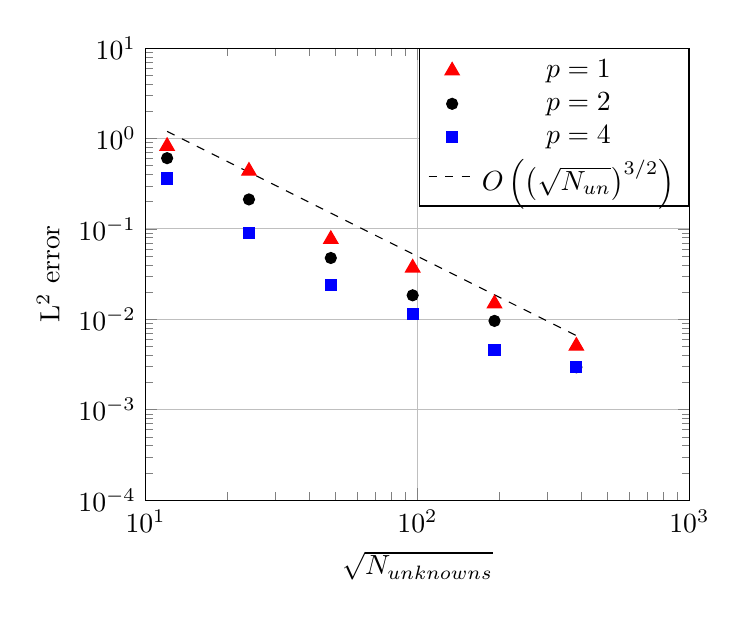
\begin{tikzpicture}
  \begin{axis}[
    width=0.7\textwidth,
    %height=0.9\textwidth,
    grid=major,
    xlabel={$\sqrt{\text{N}_\text{unknowns}}$},
    ylabel={L$^2$ error},
  	xmode=log,
  	ymode=log,
  	xmin=10,xmax=1e3,
  	ymin=1e-4,ymax=1e1,
  	legend style={at={(1.0,1.0)},anchor=north east},
  	]

\addplot[mark=triangle*, only marks, mark size=3, draw=red, mark options={solid, fill=red}] table[row sep=crcr] {
12 0.822493 \\
24 0.43734036 \\
48 0.076831588 \\
96 0.037120875 \\
192 0.014887499 \\
384 0.0050662591 \\};
\addlegendentry{$p=1$}
\addplot[mark=*, mark size=2, only marks, draw=black, mark options={solid, fill=black}] table[row sep=crcr] {
12 0.60652325 \\
24 0.21194424 \\
48 0.047687556 \\
96 0.018428546 \\
192 0.009601399 \\
384 0.0029490701 \\};
\addlegendentry{$p=2$}
\addplot[mark=square*, only marks, mark size=2, draw=blue, mark options={solid, fill=blue}] table[row sep=crcr] {
12 0.36159159 \\
24 0.090767945 \\
48 0.02399935 \\
96 0.011502376 \\
192 0.0045548581 \\
384 0.0029490701 \\};
\addlegendentry{$p=4$}

\addplot[dashed,black] table[row sep=crcr] {
12 1.2 \\
384 0.0066 \\};
\addlegendentry{$O \left(\left(\sqrt{N_\text{un}} \right)^{3/2} \right)$}

  \end{axis}
\end{tikzpicture}
\caption{L$^2$-norm of the errors from the manufactured solution and reference lines, where $N_\text{unknowns}~=~N_\text{cells}(p~+~1)^2$.}
\label{fig:RZMMSDiscontRp2S12g2Errors}
\end{figure}

\FloatBarrier

%%%%%%%%%%%%%%%%%%%%%%%%%%%%%%%%%%%%%%%
{\color{red}
\subsection{Lumping}
We may get into this...
}

%%%%%%%%%%%%%%%%%%%%%%%%%%%%%%%%%%%%%%%
{\color{red}
\subsection{Diffusion Synthetic Acceleration}
We may get into this...
}


%%%%%%%%%%%%%%%%%%%%%%%%%%%%%%%%%%%%%%%
\subsection{Axisymmetry Preservation}
\label{sec:AxisymmetryPreservations}
Numerically solving the radiation transport equation for a spherically shaped problem using spherical geometry is a very reasonable idea. However, it is also necessary to solve a spherical problem using cylindrical geometry. One particular application of the transport equation is coupling it to the hydrodynamics equations to solve radiation-hydrodynamics problems. Numerical modeling hydrodynamics problems in cylindrical geometry is common~\cite{DobrevHOAxisymmetric} so we too must demonstrate the ability to model spherical problems using cylindrical geometry.
We want \RZ\ geometry to solve and preserve 1-dimensional spherical solutions. We use MMS to solve a 1-D spherical problem using the \RZ\ geometry spatial discretization.
{\color{red}The manufactured solution is
\begin{flalign}
\psi_\text{MMS} (\rho) & = \sin(\pi \rho) + 2 -\rho,
\end{flalign}
%
\noindent where $\rho = \sqrt{r^2 + z^2}$ is the distance from the origin (i.e. the spherical radius). First, we integrate the streaming term by parts,
\begin{flalign}
\vec{\Omega} \vd \grad \psi & = \mu \frac{\partial \psi}{\partial r} + \frac{\mu}{r} \psi + \xi \frac{\partial \psi}{\partial r} - \frac{\mu}{r} \psi - \frac{\eta}{r} \frac{\partial \psi}{\partial \omega} \\
& = \mu \frac{\partial \psi}{\partial r} + \xi \frac{\partial \psi}{\partial z} - \frac{\eta}{r} \frac{\partial \psi}{\partial \omega}
\end{flalign}

\noindent Substituting the manufactured solution into this \RZ\ transport equation,
\begin{multline}
\mu \frac{\partial}{\partial r} \left(\sin (\pi \rho)+2-\rho \right) + \xi \frac{\partial}{\partial z} \left(\sin (\pi \rho)+2-\rho \right) \\
- \frac{\eta}{r} \frac{\partial}{\partial \omega} \left[\left(\sin (\pi \rho)+2-\rho \right) \right] + \sigma_t \left(\sin (\pi \rho)+2-\rho \right) \\
= \frac{1}{2 \pi} \sigma_s \phi_\text{MMS} + \frac{1}{2 \pi} S_0.
\end{multline}
%
\noindent Integrating $\psi_\text{MMS}$ over all directions reveals $\phi_\text{MMS}$,
\begin{multline}
\mu \frac{\partial}{\partial r} \left(\sin (\pi \rho)+2-\rho \right) + \xi \frac{\partial}{\partial z} \left(\sin (\pi \rho)+2-\rho \right) \\
- \frac{\eta}{r} \frac{\partial}{\partial \omega} \left[\left(\sin (\pi \rho)+2-\rho \right) \right] + \sigma_t \left(\sin (\pi \rho)+2-\rho \right) \\
= \sigma_s \left(\sin (\pi \rho)+2-\rho \right) + \frac{1}{2 \pi} S_0.
\end{multline}
%
\noindent We perform some simplifications,
\begin{flalign}
\frac{\partial \psi}{\partial r} & = \frac{\pi r \cos(\pi \sqrt{r^2+z^2})}{\sqrt{r^2+z^2}} - \frac{r}{\sqrt{r^2+z^2}} \\
\frac{\partial \psi}{\partial z} & = \frac{\pi z \cos(\pi \sqrt{r^2+z^2})}{\sqrt{r^2+z^2}} - \frac{r}{\sqrt{r^2+z^2}}
\end{flalign}

{\color{blue}
\begin{multline}
\mu \frac{\partial}{\partial r} \left(\sin (\pi \rho)+2-\rho \right) + \xi \frac{\partial}{\partial z} \left(\sin (\pi \rho)+2-\rho \right) \\
- \frac{\eta}{r} \frac{\partial}{\partial \omega} \left[\left(\sin (\pi \rho)+2-\rho \right) \right] + \sigma_t \left(\sin (\pi \rho)+2-\rho \right) \\
= \sigma_s \left(\sin (\pi \rho)+2-\rho \right) + \frac{1}{2 \pi} S_0.
\end{multline}
}

Because of the angular derivative in the streaming term, we reduce the influence of the direction dependence as much as possible by using higher order level-symmetric angular quadrature.
}

We evaluate the relative asymmetry by calculating the averages of all nodes at each $\rho$ value and
\begin{flalign}
\phi_\text{sym} (\rho, \theta) & = \frac{\phi_\text{code}(\rho, \theta) - \phi_\text{avg}(\rho)}{\phi_\text{avg}(\rho)},
\label{eq:RelativeAsymmetry}
\end{flalign}
%
\noindent where
\begin{flalign}
\phi_\text{avg}(\rho) & = \frac{1}{N_\text{nodes}(\rho)} \sum_{i=1}^{N_\text{nodes}(\rho)} \phi(\rho,\theta_i)
\end{flalign}
%
\noindent is the average scalar flux at all nodes at the same spherical radius $\rho=\sqrt{r^2+z^2}$.


%%%%%%%%%%%%%%%%%%%%%%%%%%%%%%%%%%%%%%%
The three traditional coordinate systems are Cartesian, cylindrical, and spherical. It is straight forward to describe a spatial position using any one of them. However, challenges arise when spatially discretizing. Specifically, angular derivatives arise inside the streaming term in cylindrical and spherical geometries. In modeling a spherical problem, it would seem best to use a spherical coordinate system to describe the spatial domain. However, there are more angular derivatives that must now be handled with a numerical scheme. Cylindrical geometry may be used in lieu of spherical coordinates to describe a spherical problem and is performed this way in some hydrodynamics calculations~\cite{DobrevHOAxisymmetric}. In this section, we demonstrate the use of \RZ\ geometry to preserve a 1-D spherical solution.

We use the method of manufactured solutions (MMS) with the manufactured solution
\begin{flalign}
\psi_\text{MMS}(r,z) & = \rho = \sqrt{r^2+z^2}.
\label{eq:RZMMSLinearRho}
\end{flalign}
%
This solution is linear in the 1-D spherical coordinate $\rho$. We solve this for $p=\{1,2,4,8\}$, using $S_N$ level symmetric angular quadrature with $N=\{4,6,8,10,12\}$, on a $1^\text{st}$- and $2^\text{nd}$-order mesh. The problem has physical parameters $\sigma_t=5.0$ and $\sigma_a=2.0$. We solve each of these problems on a LO mesh and a HO ($2^\text{nd}$-order) mesh. Sections~\ref{subsec:LOMesh}~and~\ref{subsec:HOMesh} show and discuss the results on the low-order and high-order meshes, respectively.

%%%%%%%%%%%%%%%%%%%%%%%%%%%%%%%%%%%%%%%
\subsubsection{Low-Order Mesh}
\label{subsec:LOMesh}
In this section, we observe the sensitivity of the scalar flux spherical asymmetry to changing the discrete ordinates order, finite element order, and spatial refinement on a low-order mesh. Specifically, a low-order mesh is one that has linear surfaces. The vertices of the low-order meshes used in this section are located in concentric rings of equal $\rho=\sqrt{r^2+z^2}$. The results in this section are organized as follows: comparing the discrete ordinates order for each of $p=\{1,2,4,8\}$, comparing each of $p=\{1,2,4,8\}$ for $S_8$ level symmetric angular quadrature, and mesh refinement studies for each of $p=\{1,4\}$.

Figure~\ref{fig:RZASMMSLinearRhoBrunnerp1g1r2} shows the $\phi_\text{sym}$ values calculated using Equation~\ref{eq:RelativeAsymmetry} for $1^\text{st}$-order finite elements on a $1^\text{st}$-order mesh with 120 zones for several angular quadrature discretizations. The asymmetry is plotted on a log scale. The scale colors assist in demonstrating the qualitative locations of the asymmetries. The yellow region is the least symmetric, red regions have increased symmetry, and blue regions have the most symmetry. The $\phi_\text{sym}$ solution is plotted using the same finite element shape functions as the scalar flux. There is no perceptible gain in symmetry by increasing the angular discretization order. We confirm this by plotting the asymmetry values as a function of the spherical radius (i.e., $\rho=\sqrt{r^2+z^2}$) in Figure~\ref{fig:RZASMMSLinearRhoBrunnerp1g1r2Nodes}. The spherical radial asymmetry solutions are indistinguishable between discrete ordinate orders. The location of the largest asymmetries are near the polar axis (i.e., $r=0$).

\begin{sidewaysfigure}[!htb]
\centering
\begin{subfigure}{0.33\textwidth}
\includegraphics[scale=0.3,trim={50pt 70pt 320pt 45pt},clip]{../../Research/graphics/Axisymmetry/RZASMMSLinearRhoBrunner/p1S4g1r2}
\caption{$S_4$.}
\end{subfigure}%
%\begin{subfigure}{0.2\textwidth}
%\includegraphics[scale=0.25,trim={50pt 70pt 320pt 45pt},clip]{../../Research/graphics/Axisymmetry/RZASMMSLinearRhoBrunner/p1S6g1r2}
%\caption{$S_6$.}
%\end{subfigure}%
\begin{subfigure}{0.33\textwidth}
\includegraphics[scale=0.3,trim={50pt 70pt 320pt 45pt},clip]{../../Research/graphics/Axisymmetry/RZASMMSLinearRhoBrunner/p1S8g1r2}
\caption{$S_8$.}
\end{subfigure}%
%\begin{subfigure}{0.2\textwidth}
%\includegraphics[scale=0.25,trim={50pt 70pt 320pt 45pt},clip]{../../Research/graphics/Axisymmetry/RZASMMSLinearRhoBrunner/p1S10g1r2}
%\caption{$S_{10}$.}
%\end{subfigure}%
\begin{subfigure}{0.33\textwidth}
\includegraphics[scale=0.3,trim={50pt 70pt 320pt 45pt},clip]{../../Research/graphics/Axisymmetry/RZASMMSLinearRhoBrunner/p1S12g1r2}
\caption{$S_{12}$.}
\end{subfigure}
\caption{Relative asymmetry for $1^\text{st}$-order finite elements on a $1^\text{st}$-order mesh for given order of level-symmetric angular quadrature.}
\label{fig:RZASMMSLinearRhoBrunnerp1g1r2}
\end{sidewaysfigure}

\begin{figure}[!htb]
\centering
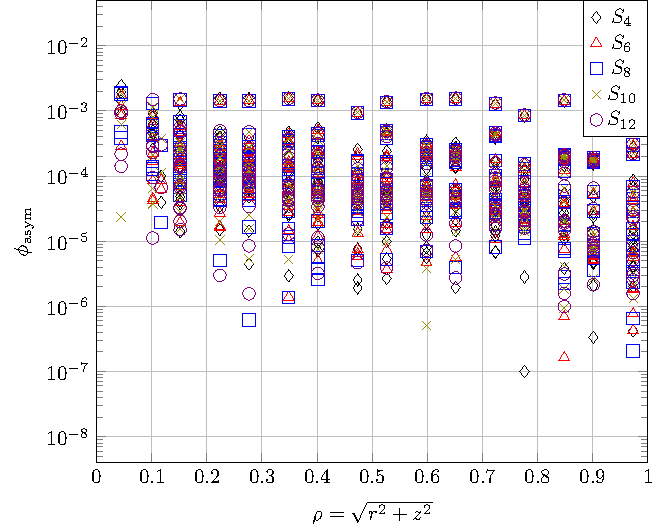
\includegraphics[scale=1]{./graphics/RZASMMSLinearRhoBrunnerp1g1r2.pdf}
\caption{Measure of the asymmetry for each finite element node for the given level-symmetric angular quadrature order for $1^\text{st}$-order DFEM and $1^\text{st}$-order mesh with 120 zones (see Figure~\ref{fig:RZASMMSLinearRhoBrunnerp1g1r2}).}
\label{fig:RZASMMSLinearRhoBrunnerp1g1r2Nodes}
\end{figure}

\begin{table}[!htb]
\centering
{\renewcommand{\arraystretch}{1.5}
\begin{tabular}{|c|c|}
\hline
$S_N$ & L$^2$ error \\\hline
$S_4$ & 0.0020941929 \\\hline
$S_6$ & 0.0020971511 \\\hline
$S_8$ & 0.0021251254 \\\hline
$S_{10}$ & 0.0021502437 \\\hline
$S_{12}$ & 0.0021700218 \\\hline
\end{tabular}}
\end{table}

\FloatBarrier

Figure~\ref{fig:RZASMMSLinearRhoBrunnerp2g1r2} shows the $\phi_\text{sym}$ values calculated using Equation~\ref{eq:RelativeAsymmetry} for $2^\text{nd}$-order finite elements on a $1^\text{st}$-order mesh with 120 zones for several angular quadrature discretizations. The asymmetry is plotted on a log scale. The scale colors assist in demonstrating the qualitative locations of the asymmetries. The yellow region is the least symmetric, red regions have increased symmetry, and blue regions have the most symmetry. The $\phi_\text{sym}$ solution is plotted using the same finite element shape functions as the scalar flux. There is a little perceptible gain in symmetry (indicated by more blue area) on the periphery by increasing the angular discretization order. However, plotting the asymmetry values as a function of the spherical radius (i.e., $\rho=\sqrt{r^2+z^2}$) in Figure~\ref{fig:RZASMMSLinearRhoBrunnerp2g1r2Nodes} shows that there may not actually be any symmetry gains --- the spherical radial asymmetry solutions are indistinguishable between discrete ordinate orders. The asymmetries are predominantly located near the origin (i.e., $\rho=\sqrt{r^2+z^2}=0$).

\begin{sidewaysfigure}[!htb]
\centering
\begin{subfigure}{0.33\textwidth}
\includegraphics[scale=0.3,trim={50pt 70pt 320pt 45pt},clip]{../../Research/graphics/Axisymmetry/RZASMMSLinearRhoBrunner/p2S4g1r2}
\caption{$S_4$.}
\end{subfigure}%
%\begin{subfigure}{0.2\textwidth}
%\includegraphics[scale=0.25,trim={50pt 70pt 320pt 45pt},clip]{../../Research/graphics/Axisymmetry/RZASMMSLinearRhoBrunner/p2S6g1r2}
%\caption{$S_6$.}
%\end{subfigure}%
\begin{subfigure}{0.33\textwidth}
\includegraphics[scale=0.3,trim={50pt 70pt 320pt 45pt},clip]{../../Research/graphics/Axisymmetry/RZASMMSLinearRhoBrunner/p2S8g1r2}
\caption{$S_8$.}
\end{subfigure}%
%\begin{subfigure}{0.2\textwidth}
%\includegraphics[scale=0.25,trim={50pt 70pt 320pt 45pt},clip]{../../Research/graphics/Axisymmetry/RZASMMSLinearRhoBrunner/p2S10g1r2}
%\caption{$S_10$.}
%\end{subfigure}%
\begin{subfigure}{0.33\textwidth}
\includegraphics[scale=0.3,trim={50pt 70pt 320pt 45pt},clip]{../../Research/graphics/Axisymmetry/RZASMMSLinearRhoBrunner/p2S12g1r2}
\caption{$S_{12}$.}
\end{subfigure}
\caption{Relative asymmetry for $2^\text{st}$-order finite elements on a $1^\text{st}$-order mesh for given order of level-symmetric angular quadrature.}
\label{fig:RZASMMSLinearRhoBrunnerp2g1r2}
\end{sidewaysfigure}

\begin{figure}[!htb]
\centering
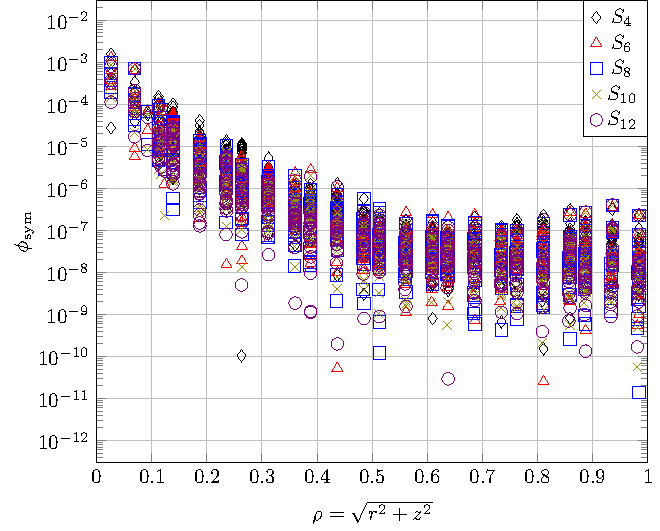
\includegraphics[scale=1]{./graphics/RZASMMSLinearRhoBrunnerp2g1r2.pdf}
\caption{Measure of the asymmetry for each finite element node for the given level-symmetric angular quadrature order for $2^\text{nd}$-order DFEM and $1^\text{st}$-order mesh with 120 zones (see Figure~\ref{fig:RZASMMSLinearRhoBrunnerp2g1r2}).}
\label{fig:RZASMMSLinearRhoBrunnerp2g1r2Nodes}
\end{figure}

\begin{table}[!htb]
\centering
{\renewcommand{\arraystretch}{1.5}
\begin{tabular}{|c|c|}
\hline
$S_N$ & L$^2$ error \\\hline
$S_4$ & 0.00053016665 \\\hline
$S_6$ & 0.00050896038 \\\hline
$S_8$ & 0.00050561127 \\\hline
$S_{10}$ & 0.00050450878 \\\hline
$S_{12}$ & 0.00050268774 \\\hline
\end{tabular}}
\end{table}

\FloatBarrier

Figure~\ref{fig:RZASMMSLinearRhoBrunnerp4g1r2} shows the $\phi_\text{sym}$ values calculated using Equation~\ref{eq:RelativeAsymmetry} for $4^\text{th}$-order finite elements on a $1^\text{st}$-order mesh with 120 zones for several angular quadrature discretizations. The asymmetry is plotted on a log scale. The scale colors assist in demonstrating the qualitative locations of the asymmetries. The yellow region is the least symmetric, red regions have increased symmetry, and blue regions have the most symmetry. The $\phi_\text{sym}$ solution is plotted using the same finite element shape functions as the scalar flux. There is no perceptible gain in symmetry by increasing the angular discretization order. This is confirmed by plotting the asymmetry values as a function of the spherical radius (i.e., $\rho=\sqrt{r^2+z^2}$) in Figure~\ref{fig:RZASMMSLinearRhoBrunnerp4g1r2Nodes}. Unlike Figure~\ref{fig:RZASMMSLinearRhoBrunnerp2g1r2}, the asymmetry of the scalar flux appears to be a function of the spherical radius, $\rho$.

\begin{sidewaysfigure}[!htb]
\centering
\begin{subfigure}{0.33\textwidth}
\includegraphics[scale=0.3,trim={50pt 70pt 320pt 45pt},clip]{../../Research/graphics/Axisymmetry/RZASMMSLinearRhoBrunner/p4S4g1r2}
\caption{$S_4$.}
\end{subfigure}%
%\begin{subfigure}{0.2\textwidth}
%\includegraphics[scale=0.25,trim={50pt 70pt 320pt 45pt},clip]{../../Research/graphics/Axisymmetry/RZASMMSLinearRhoBrunner/p4S6g1r2}
%\caption{$S_6$.}
%\end{subfigure}%
\begin{subfigure}{0.33\textwidth}
\includegraphics[scale=0.3,trim={50pt 70pt 320pt 45pt},clip]{../../Research/graphics/Axisymmetry/RZASMMSLinearRhoBrunner/p4S8g1r2}
\caption{$S_8$.}
\end{subfigure}%
%\begin{subfigure}{0.2\textwidth}
%\includegraphics[scale=0.25,trim={50pt 70pt 320pt 45pt},clip]{../../Research/graphics/Axisymmetry/RZASMMSLinearRhoBrunner/p4S10g1r2}
%\caption{$S_{10}$.}
%\end{subfigure}%
\begin{subfigure}{0.33\textwidth}
\includegraphics[scale=0.3,trim={50pt 70pt 320pt 45pt},clip]{../../Research/graphics/Axisymmetry/RZASMMSLinearRhoBrunner/p4S12g1r2}
\caption{$S_{12}$.}
\end{subfigure}
\caption{Relative asymmetry for $4^\text{st}$-order finite elements on a $1^\text{st}$-order mesh for given order of level-symmetric angular quadrature.}
\label{fig:RZASMMSLinearRhoBrunnerp4g1r2}
\end{sidewaysfigure}

\begin{figure}[!htb]
\centering
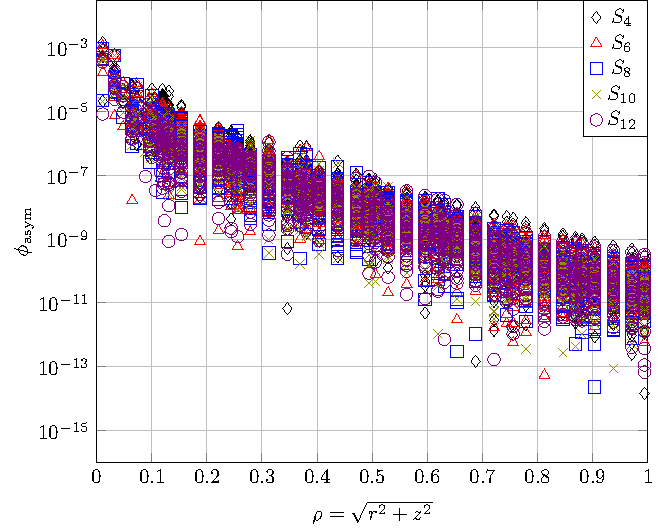
\includegraphics[scale=1]{./graphics/RZASMMSLinearRhoBrunnerp4g1r2.pdf}
\caption{Measure of the asymmetry for each finite element node for the given level-symmetric angular quadrature order for $4^\text{th}$-order DFEM and $1^\text{st}$-order mesh with 120 zones (see Figure~\ref{fig:RZASMMSLinearRhoBrunnerp4g1r2}).}
\label{fig:RZASMMSLinearRhoBrunnerp4g1r2Nodes}
\end{figure}

\begin{table}[!htb]
\centering
{\renewcommand{\arraystretch}{1.5}
\begin{tabular}{|c|c|}
\hline
$S_N$ & L$^2$ error \\\hline
$S_4$ & 0.00010668759 \\\hline
$S_6$ & 0.00010001654 \\\hline
$S_8$ & 7.8171296e-06 \\\hline
$S_{10}$ & 9.8179924e-05 \\\hline
$S_{12}$ & 9.7617814e-05 \\\hline
\end{tabular}}
\end{table}

\FloatBarrier

Figure~\ref{fig:RZASMMSLinearRhoBrunnerp8g1r2} shows the $\phi_\text{sym}$ values calculated using Equation~\ref{eq:RelativeAsymmetry} for $8^\text{th}$-order finite elements on a $1^\text{st}$-order mesh with 120 zones for several angular quadrature discretizations. The asymmetry is plotted on a log scale. The scale colors assist in demonstrating the qualitative locations of the asymmetries. The yellow region is the least symmetric, red regions have increased symmetry, and blue regions have the most symmetry. The $\phi_\text{sym}$ solution is plotted using the same finite element shape functions as the scalar flux. There is no perceptible gain in symmetry by increasing the angular discretization order. However, Figure~\ref{fig:RZASMMSLinearRhoBrunnerp8g1r2Nodes} shows there is a slight increase in symmetry from $S_4$ for $\rho \geq 0.7$. Similar to Figure~\ref{fig:RZASMMSLinearRhoBrunnerp4g1r2}, the asymmetry of the scalar flux appears to be a function of the spherical radius, $\rho$.

\begin{sidewaysfigure}[!htb]
\centering
\begin{subfigure}{0.33\textwidth}
\includegraphics[scale=0.3,trim={50pt 70pt 320pt 45pt},clip]{../../Research/graphics/Axisymmetry/RZASMMSLinearRhoBrunner/p8S4g1r2}
\caption{$S_4$.}
\end{subfigure}%
%\begin{subfigure}{0.2\textwidth}
%\includegraphics[scale=0.25,trim={50pt 70pt 320pt 45pt},clip]{../../Research/graphics/Axisymmetry/RZASMMSLinearRhoBrunner/p8S6g1r2}
%\caption{$S_6$.}
%\end{subfigure}%
\begin{subfigure}{0.33\textwidth}
\includegraphics[scale=0.3,trim={50pt 70pt 320pt 45pt},clip]{../../Research/graphics/Axisymmetry/RZASMMSLinearRhoBrunner/p8S8g1r2}
\caption{$S_8$.}
\end{subfigure}%
%\begin{subfigure}{0.2\textwidth}
%\includegraphics[scale=0.25,trim={50pt 70pt 320pt 45pt},clip]{../../Research/graphics/Axisymmetry/RZASMMSLinearRhoBrunner/p8S10g1r2}
%\caption{$S_{10}$.}
%\end{subfigure}%
\begin{subfigure}{0.33\textwidth}
\includegraphics[scale=0.3,trim={50pt 70pt 320pt 45pt},clip]{../../Research/graphics/Axisymmetry/RZASMMSLinearRhoBrunner/p8S10g1r2}
\caption{$S_{12}$.}
\end{subfigure}
\caption{Relative asymmetry for $8^\text{st}$-order finite elements on a $1^\text{st}$-order mesh for given order of level-symmetric angular quadrature.}
\label{fig:RZASMMSLinearRhoBrunnerp8g1r2}
\end{sidewaysfigure}

\begin{figure}[!htb]
\centering
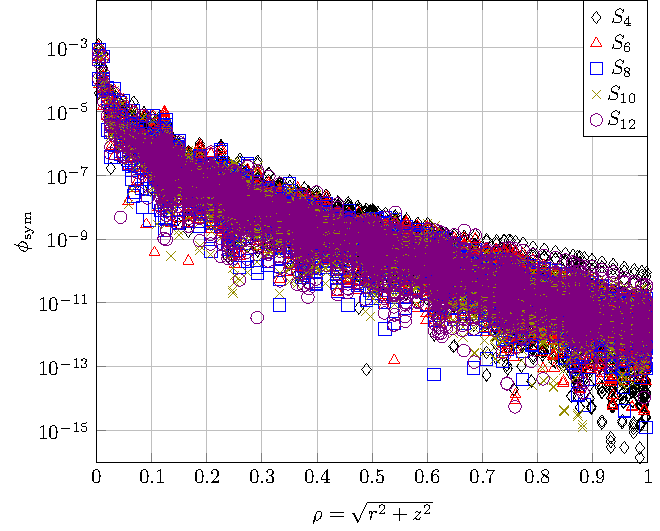
\includegraphics[scale=1]{./graphics/RZASMMSLinearRhoBrunnerp8g1r2.pdf}
\caption{Measure of the asymmetry for each finite element node for the given level-symmetric angular quadrature order for $8^\text{th}$-order DFEM and $1^\text{st}$-order mesh with 120 zones (see Figure~\ref{fig:RZASMMSLinearRhoBrunnerp8g1r2}).}
\label{fig:RZASMMSLinearRhoBrunnerp8g1r2Nodes}
\end{figure}

\begin{table}[!htb]
\centering
{\renewcommand{\arraystretch}{1.5}
\begin{tabular}{|c|c|}
\hline
$S_N$ & L$^2$ error \\\hline
$S_4$ & 1.4392389e-05 \\\hline
$S_6$ & 1.3173359e-05 \\\hline
$S_8$ & 1.2895207e-05 \\\hline
$S_{10}$ & 1.2783353e-05 \\\hline
$S_{12}$ & 1.2700264e-05 \\\hline
\end{tabular}}
\end{table}

\FloatBarrier

Figure~\ref{fig:RZASMMSLinearRhoBrunnerS8g1r2CompareP} shows the $\phi_\text{sym}$ values calculated using Equation~\ref{eq:RelativeAsymmetry} for $p=\{1,2,4\}$ finite elements on a $2^\text{nd}$-order mesh with 120 zones with $S_8$ level-symmetric angular quadrature repeated from Figures~\ref{fig:RZASMMSLinearRhoBrunnerp1g1r2},~\ref{fig:RZASMMSLinearRhoBrunnerp2g1r2},~and~\ref{fig:RZASMMSLinearRhoBrunnerp4g1r2} and plotted on the same scale. Increasing the finite element order provides significant gains in symmetry shown by the reduction in yellow regions and increase in blue regions. We corroborate these results by plotting the asymmetry values as a function of the spherical radius (i.e., $\rho=\sqrt{r^2+z^2}$) in Figure~\ref{fig:RZASMMSLinearRhoBrunnerS8g1r2Nodes}. It is evident that increasing the finite element order provides gains in spherical symmetry.

\begin{sidewaysfigure}[!htb]
\centering
\begin{subfigure}{0.33\textwidth}
\includegraphics[scale=0.3,trim={50pt 70pt 320pt 45pt},clip]{../../Research/graphics/Axisymmetry/RZASMMSLinearRhoBrunner/p1S8g1r2CompP}
\caption{$p=1$.}
\end{subfigure}%
\begin{subfigure}{0.33\textwidth}
\includegraphics[scale=0.3,trim={50pt 70pt 320pt 45pt},clip]{../../Research/graphics/Axisymmetry/RZASMMSLinearRhoBrunner/p2S8g1r2CompP}
\caption{$p=2$.}
\end{subfigure}%
\begin{subfigure}{0.33\textwidth}
\includegraphics[scale=0.3,trim={50pt 70pt 320pt 45pt},clip]{../../Research/graphics/Axisymmetry/RZASMMSLinearRhoBrunner/p4S8g1r2CompP}
\caption{$p=4$.}
\end{subfigure}
\caption{Relative asymmetry for $p=\{1,2,4\}$ finite elements on a $1^\text{st}$-order mesh with 120 zones for $S_8$ level-symmetric angular quadrature.}
\label{fig:RZASMMSLinearRhoBrunnerS8g1r2CompareP}
\end{sidewaysfigure}

\begin{figure}[!htb]
\centering
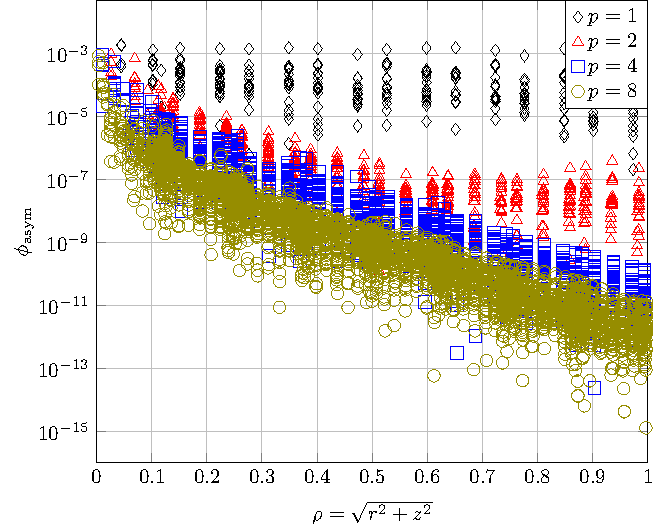
\includegraphics[scale=1]{./graphics/RZASMMSLinearRhoBrunnerS8g1r2.pdf}
\caption{Measure of the asymmetry for each finite element node for the given finite element order using $S_8$ level-symmetric angular quadrature on a $1^\text{st}$-order mesh with 120 zones (see Figure~\ref{fig:RZASMMSLinearRhoBrunnerS8g1r2CompareP}).}
\label{fig:RZASMMSLinearRhoBrunnerS8g1r2Nodes}
\end{figure}

\begin{table}[!htb]
\centering
{\renewcommand{\arraystretch}{1.5}
\begin{tabular}{|c|c|}
\hline
$p$ & L$^2$ error \\\hline
1 & 0.0021251254 \\\hline
2 & 0.00050561127 \\\hline
4 & 7.8171296e-06 \\\hline
\end{tabular}}
\end{table}

\FloatBarrier

We also investigated the symmetry preservation my performing sequential mesh refinements for $p=1$ with $S_8$ level-symmetric angular quadrature. Figures~\ref{fig:RZASMMSLinearRhoBrunnerp1S8g1Part1}~and~\ref{fig:RZASMMSLinearRhoBrunnerp1S8g1Part2} show the first several mesh refinement steps. The asymmetry is plotted on a log scale. The scale colors assist in demonstrating the qualitative locations of the asymmetries. The yellow region is the least symmetric, red regions have increased symmetry, and blue regions have the most symmetry. The $\phi_\text{sym}$ solution is plotted using the same finite element shape functions as the scalar flux. There is some gain (a few orders of magnitude) in symmetry by refining the $1^\text{st}$-order mesh. We observe large regions of $\phi_\text{sym}$ changing from yellow to red through the mesh refinement. Plotting the symmetry values as a function of the spherical radius (i.e., $\rho=\sqrt{r^2+z^2}$) in Figure~\ref{fig:RZASMMSLinearRhoBrunnerp1S8g1Nodes} shows that there is some symmetry gain by refining the mesh. The largest asymmetry magnitude of the scalar flux is near the polar axis (i.e. $r=0$) as previously seen in Figure~\ref{fig:RZASMMSLinearRhoBrunnerp1g1r2}.

\begin{sidewaysfigure}[!htb]
\centering
\begin{subfigure}{0.33\textwidth}
\includegraphics[scale=0.3,trim={50pt 70pt 320pt 45pt},clip]{../../Research/graphics/Axisymmetry/RZASMMSLinearRhoBrunner/p1S8g1r0CompR}
\caption{$N_\text{zones}=6$.}
\end{subfigure}%
\begin{subfigure}{0.33\textwidth}
\includegraphics[scale=0.3,trim={50pt 70pt 320pt 45pt},clip]{../../Research/graphics/Axisymmetry/RZASMMSLinearRhoBrunner/p1S8g1r1CompR}
\caption{$N_\text{zones}=28$.}
\end{subfigure}%
\begin{subfigure}{0.33\textwidth}
\includegraphics[scale=0.3,trim={50pt 70pt 320pt 45pt},clip]{../../Research/graphics/Axisymmetry/RZASMMSLinearRhoBrunner/p1S8g1r2CompR}
\caption{$N_\text{zones}=120$.}
\end{subfigure}
\caption{Relative asymmetry for $p=1$ finite elements on a $1^\text{st}$-order mesh for $S_8$ level-symmetric angular quadrature for $N_\text{zones}=\{6,28,120\}$.}
\label{fig:RZASMMSLinearRhoBrunnerp1S8g1Part1}
\end{sidewaysfigure}

\begin{sidewaysfigure}[!htb]
\centering
\begin{subfigure}{0.33\textwidth}
\includegraphics[scale=0.3,trim={50pt 70pt 320pt 45pt},clip]{../../Research/graphics/Axisymmetry/RZASMMSLinearRhoBrunner/p1S8g1r3CompR}
\caption{$N_\text{zones}=496$.}
\end{subfigure}%
\begin{subfigure}{0.33\textwidth}
\includegraphics[scale=0.3,trim={50pt 70pt 320pt 45pt},clip]{../../Research/graphics/Axisymmetry/RZASMMSLinearRhoBrunner/p1S8g1r4CompR}
\caption{$N_\text{zones}=2016$.}
\end{subfigure}%
\begin{subfigure}{0.33\textwidth}
\includegraphics[scale=0.3,trim={50pt 70pt 320pt 45pt},clip]{../../Research/graphics/Axisymmetry/RZASMMSLinearRhoBrunner/p1S8g1r5CompR}
\caption{$N_\text{zones}=8128$.}
\end{subfigure}
\caption{Relative asymmetry for $p=1$ finite elements on a $1^\text{st}$-order mesh for $S_8$ level-symmetric angular quadrature for $N_\text{zones}=\{496,2016,8128\}$; mesh overlay may be removed for clarity.}
\label{fig:RZASMMSLinearRhoBrunnerp1S8g1Part2}
\end{sidewaysfigure}

\begin{figure}[!htb]
\centering
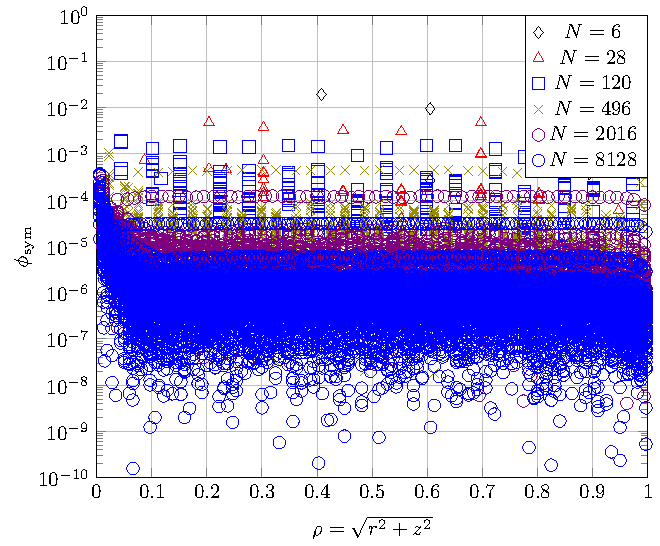
\includegraphics[scale=1]{./graphics/RZASMMSLinearRhoBrunnerp1S8g1.pdf}
\caption{Measure of the asymmetry for each finite element node for $1^\text{th}$-order finite elements using $S_8$ level-symmetric angular quadrature on a $1^\text{st}$-order mesh with various number of zones (see Figures~\ref{fig:RZASMMSLinearRhoBrunnerp1S8g1Part1}-\ref{fig:RZASMMSLinearRhoBrunnerp1S8g1Part2}).}
\label{fig:RZASMMSLinearRhoBrunnerp1S8g1Nodes}
\end{figure}

\begin{table}[!htb]
\centering
{\renewcommand{\arraystretch}{1.5}
\begin{tabular}{|c|c|}
\hline
$N_\text{unknowns}$ & L$^2$ error \\\hline
$6$ & 0.041323342 \\\hline
$28$ & 0.0088741901 \\\hline
$120$ & 0.0021251254 \\\hline
$496$ & 0.00045204233 \\\hline
$2016$ & 8.8560131e-05 \\\hline
$8128$ & 1.6559953e-05 \\\hline
\end{tabular}}
\end{table}

\FloatBarrier

We also investigated the symmetry preservation my performing sequential mesh refinements for $p=4$ with $S_8$ level-symmetric angular quadrature. Figures~\ref{fig:RZASMMSLinearRhoBrunnerp4S8g1Part1}~and~\ref{fig:RZASMMSLinearRhoBrunnerp4S8g1Part2} show the first several mesh refinement steps. The asymmetry is plotted on a log scale. The scale colors assist in demonstrating the qualitative locations of the asymmetries. The yellow region is the least symmetric, red regions have increased symmetry, and blue regions have the most symmetry. The $\phi_\text{sym}$ solution is plotted using the same finite element shape functions as the scalar flux. There is tremendous gain (many orders of magnitude) in symmetry by refining the $1^\text{st}$-order mesh. We observe large regions of $\phi_\text{sym}$ changing from yellow to red to blue throughout the mesh refinement. Plotting the symmetry values as a function of the spherical radius (i.e., $\rho=\sqrt{r^2+z^2}$) in Figure~\ref{fig:RZASMMSLinearRhoBrunnerp4S8g1Nodes} confirms the substantial symmetry gain by refining the mesh. The largest asymmetry magnitude of the scalar flux remains near the orign (i.e. $\rho=\sqrt{r^2+z^2}=0$) as previously seen, but also remains prevalent in the discrete ordinates directions as though there were ray effects.

\begin{sidewaysfigure}[!htb]
\centering
\begin{subfigure}{0.33\textwidth}
\includegraphics[scale=0.3,trim={50pt 70pt 320pt 45pt},clip]{../../Research/graphics/Axisymmetry/RZASMMSLinearRhoBrunner/p4S8g1r0CompR}
\caption{$N_\text{zones}=6$.}
\end{subfigure}%
\begin{subfigure}{0.33\textwidth}
\includegraphics[scale=0.3,trim={50pt 70pt 320pt 45pt},clip]{../../Research/graphics/Axisymmetry/RZASMMSLinearRhoBrunner/p4S8g1r1CompR}
\caption{$N_\text{zones}=28$.}
\end{subfigure}%
\begin{subfigure}{0.33\textwidth}
\includegraphics[scale=0.3,trim={50pt 70pt 320pt 45pt},clip]{../../Research/graphics/Axisymmetry/RZASMMSLinearRhoBrunner/p4S8g1r2CompR}
\caption{$N_\text{zones}=120$.}
\end{subfigure}
\caption{Relative asymmetry for $p=4$ finite elements on a $1^\text{st}$-order mesh for $S_8$ level-symmetric angular quadrature for $N_\text{zones}=\{6,28,120\}$.}
\label{fig:RZASMMSLinearRhoBrunnerp4S8g1Part1}
\end{sidewaysfigure}

\begin{sidewaysfigure}[!htb]
\centering
\begin{subfigure}{0.33\textwidth}
\includegraphics[scale=0.3,trim={50pt 70pt 320pt 45pt},clip]{../../Research/graphics/Axisymmetry/RZASMMSLinearRhoBrunner/p4S8g1r3CompR}
\caption{$N_\text{zones}=496$.}
\end{subfigure}%
\begin{subfigure}{0.33\textwidth}
\includegraphics[scale=0.3,trim={50pt 70pt 320pt 45pt},clip]{../../Research/graphics/Axisymmetry/RZASMMSLinearRhoBrunner/p4S8g1r4CompR}
\caption{$N_\text{zones}=2016$.}
\end{subfigure}%
\begin{subfigure}{0.33\textwidth}
\includegraphics[scale=0.3,trim={50pt 70pt 320pt 45pt},clip]{../../Research/graphics/Axisymmetry/RZASMMSLinearRhoBrunner/p4S8g1r5CompR}
\caption{$N_\text{zones}=8128$.}
\end{subfigure}
\caption{Relative asymmetry for $p=4$ finite elements on a $1^\text{st}$-order mesh for $S_8$ level-symmetric angular quadrature for $N_\text{zones}=\{496,2016,8128\}$; mesh overlay may be removed for clarity.}
\label{fig:RZASMMSLinearRhoBrunnerp4S8g1Part2}
\end{sidewaysfigure}

\begin{figure}[!htb]
\centering
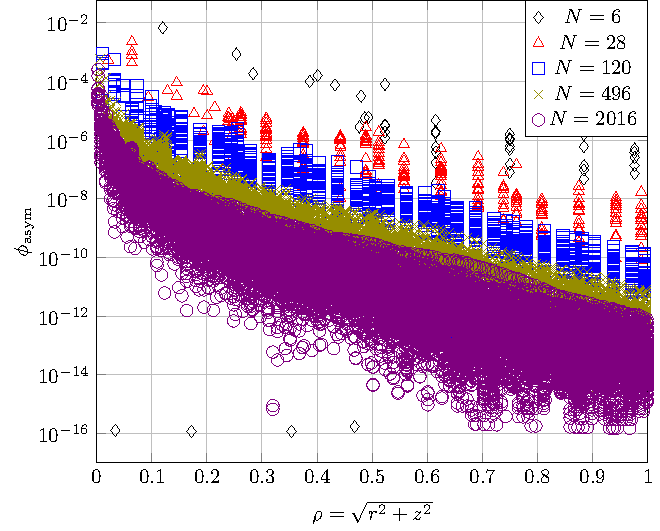
\includegraphics[scale=1]{./graphics/RZASMMSLinearRhoBrunnerp4S8g1.pdf}
\caption{Measure of the asymmetry for each finite element node for $4^\text{th}$-order finite elements using $S_8$ level-symmetric angular quadrature on a $1^\text{st}$-order mesh with various number of zones (see Figures~\ref{fig:RZASMMSLinearRhoBrunnerp4S8g1Part1}-\ref{fig:RZASMMSLinearRhoBrunnerp4S8g1Part2}).}
\label{fig:RZASMMSLinearRhoBrunnerp4S8g1Nodes}
\end{figure}

\begin{table}[!htb]
\centering
{\renewcommand{\arraystretch}{1.5}
\begin{tabular}{|c|c|}
\hline
$N_\text{unknowns}$ & L$^2$ error \\\hline
$6$ & 0.0017878942 \\\hline
$28$ & 9.8887338e-05 \\\hline
$120$ & 7.8171296e-06 \\\hline
$496$ & 6.2560514e-07 \\\hline
$2016$ & 4.7915253e-08 \\\hline
$8128$ & 3.4625793e-09 \\\hline
\end{tabular}}
\end{table}


%%%%%%%%%%%%%%%%%%%%%%%%%%%%%%%%%%%%%%%
%%%%%%%%%%%%%%%%%%%%%%%%%%%%%%%%%%%%%%%
%%%%%%%%%%%%%%%%%%%%%%%%%%%%%%%%%%%%%%%
%%%%%%%%%%%%%%%%%%%%%%%%%%%%%%%%%%%%%%%
\FloatBarrier

%%%%%%%%%%%%%%%%%%%%%%%%%%%%%%%%%%%%%%%
\subsubsection{High-Order Mesh}
\label{subsec:HOMesh}
Now, we perform the same asymmetry analysis using a high-order mesh. In this section, we observe the sensitivity of the scalar flux spherical asymmetry to changing the discrete ordinates order, finite element order, and spatial refinement on a high-order mesh. A high-order mesh is one that has curved polynomial surfaces. Specifically, we use $2^\text{nd}$-order meshes here. The vertices of the $2^\text{nd}$-order meshes used in this section are located in concentric rings of equal $rho=\sqrt{r^2+z^2}$, including the midpoint vertices. The results in this section are organized as follows: comparing the discrete ordinates order for each of $p=\{1,2,4\}$, comparing each of $p=\{1,2,4\}$ for $S_8$ level symmetric angular quadrature, mesh refinement studies for each of $p=\{1,4\}$, and comparing the discrete ordinates refinement on the most refined spatial mesh.

Figure~\ref{fig:RZASMMSLinearRhoBrunnerp1g2r2} shows the $\phi_\text{sym}$ values calculated using Equation~\ref{eq:RelativeAsymmetry} for $1^\text{st}$-order finite elements on a $2^\text{nd}$-order mesh with 120 zones for several angular quadrature discretizations. The asymmetry is plotted on a log scale. The scale colors assist in demonstrating the qualitative locations of the asymmetries. The yellow region is the least symmetric, red regions have increased symmetry, and blue regions have the most symmetry. The $\phi_\text{sym}$ solution is plotted using the same finite element shape functions as the scalar flux. There is no perceptible gain in symmetry by increasing the angular discretization order. We confirm this by plotting the asymmetry values as a function of the spherical radius (i.e., $\rho=\sqrt{r^2+z^2}$) in Figure~\ref{fig:RZASMMSLinearRhoBrunnerp1g2r2Nodes}. The spherical radial asymmetry solutions are indistinguishable between discrete ordinate orders.

\begin{sidewaysfigure}[!htb]
\centering
\begin{subfigure}{0.33\textwidth}
\includegraphics[scale=0.3,trim={50pt 70pt 320pt 45pt},clip]{../../Research/graphics/Axisymmetry/RZASMMSLinearRhoBrunner/p1S4g2r2}
\caption{$S_4$.}
\end{subfigure}%
%\begin{subfigure}{0.2\textwidth}
%\includegraphics[scale=0.25,trim={50pt 70pt 320pt 45pt},clip]{../../Research/graphics/Axisymmetry/RZASMMSLinearRhoBrunner/p1S6g2r2}
%\caption{$S_6$.}
%\end{subfigure}%
\begin{subfigure}{0.33\textwidth}
\includegraphics[scale=0.3,trim={50pt 70pt 320pt 45pt},clip]{../../Research/graphics/Axisymmetry/RZASMMSLinearRhoBrunner/p1S8g2r2}
\caption{$S_8$.}
\end{subfigure}%
%\begin{subfigure}{0.2\textwidth}
%\includegraphics[scale=0.25,trim={50pt 70pt 320pt 45pt},clip]{../../Research/graphics/Axisymmetry/RZASMMSLinearRhoBrunner/p1S10g2r2}
%\caption{$S_{10}$.}
%\end{subfigure}%
\begin{subfigure}{0.33\textwidth}
\includegraphics[scale=0.3,trim={50pt 70pt 320pt 45pt},clip]{../../Research/graphics/Axisymmetry/RZASMMSLinearRhoBrunner/p1S12g2r2}
\caption{$S_{12}$.}
\end{subfigure}
\caption{Relative asymmetry for $1^\text{st}$-order finite elements on a $2^\text{nd}$-order mesh for given order of level-symmetric angular quadrature.}
\label{fig:RZASMMSLinearRhoBrunnerp1g2r2}
\end{sidewaysfigure}

\begin{figure}[!htb]
\centering
\includegraphics[scale=1]{./graphics/RZASMMSLinearRhoBrunnerp1g2r2.pdf}
\caption{Measure of the asymmetry for each finite element node for the given level-symmetric angular quadrature order for $1^\text{st}$-order DFEM and $2^\text{nd}$-order mesh with 120 zones (see Figure~\ref{fig:RZASMMSLinearRhoBrunnerp1g2r2}).}
\label{fig:RZASMMSLinearRhoBrunnerp1g2r2Nodes}
\end{figure}

\begin{table}[!htb]
\centering
{\renewcommand{\arraystretch}{1.5}
\begin{tabular}{|c|c|}
\hline
$NS_N$ & L$^2$ error \\\hline
$S_4$ & 0.00064411998 \\\hline
$S_6$ & 0.00069161191 \\\hline
$S_8$ & 0.00071301712 \\\hline
$S_{10}$ & 0.0007189547 \\\hline
$S_{12}$ & 0.0007243029 \\\hline
\end{tabular}}
\end{table}

\begin{figure}[!htb]
\centering
\begin{tikzpicture}
  \begin{axis}[
    %width=0.9\textwidth,
    %height=0.9\textwidth,
    grid=major,
    xlabel={$S_N$},
    ylabel={L$^2$ error},
  	%xmode=log,
  	ymode=log,
  	xmin=4,xmax=12,
  	ymin=1e-4,ymax=1e-3,
  	]
\addplot[mark=*, mark size=2, draw=black, mark options={solid, fill=black}] table[row sep=crcr] {
4 0.00064411998 \\
6 0.00069161191 \\
8 0.00071301712 \\
10 0.0007189547 \\
12 0.0007243029 \\};

  \end{axis}
\end{tikzpicture}
\caption{Accuracy of solutions for given angular quadrature using $p=1$ on a $2^\text{nd}$-order mesh with 120 zones.}
\label{fig:RZASMMSLinearRhoBrunnerp1g2r2Accuracy}
\end{figure}

\FloatBarrier

Figure~\ref{fig:RZASMMSLinearRhoBrunnerp2g2r2} shows the $\phi_\text{sym}$ values calculated using Equation~\ref{eq:RelativeAsymmetry} for $2^\text{nd}$-order finite elements on a $2^\text{nd}$-order mesh with 120 zones for several angular quadrature discretizations. The asymmetry is plotted on a log scale. The scale colors assist in demonstrating the qualitative locations of the asymmetries. The yellow region is the least symmetric, red regions have increased symmetry, and blue regions have the most symmetry. The $\phi_\text{sym}$ solution is plotted using the same finite element shape functions as the scalar flux. There is very little perceptible gain in symmetry near the equator (i.e., $z=0$) by increasing the angular discretization order. However, plotting the asymmetry values as a function of the spherical radius (i.e., $\rho=\sqrt{r^2+z^2}$) in Figure~\ref{fig:RZASMMSLinearRhoBrunnerp2g2r2Nodes} shows that there may not actually be any symmetry gains --- the spherical radial asymmetry solutions are indistinguishable between discrete ordinate orders. The asymmetries are predominantly located near the polar axis (i.e., $r=0$).

\begin{sidewaysfigure}[!htb]
\centering
\begin{subfigure}{0.33\textwidth}
\includegraphics[scale=0.3,trim={50pt 70pt 320pt 45pt},clip]{../../Research/graphics/Axisymmetry/RZASMMSLinearRhoBrunner/p2S4g2r2}
\caption{$S_4$.}
\end{subfigure}%
%\begin{subfigure}{0.2\textwidth}
%\includegraphics[scale=0.25,trim={50pt 70pt 320pt 45pt},clip]{../../Research/graphics/Axisymmetry/RZASMMSLinearRhoBrunner/p2S6g2r2}
%\caption{$S_6$.}
%\end{subfigure}%
\begin{subfigure}{0.33\textwidth}
\includegraphics[scale=0.3,trim={50pt 70pt 320pt 45pt},clip]{../../Research/graphics/Axisymmetry/RZASMMSLinearRhoBrunner/p2S8g2r2}
\caption{$S_8$.}
\end{subfigure}%
%\begin{subfigure}{0.2\textwidth}
%\includegraphics[scale=0.25,trim={50pt 70pt 320pt 45pt},clip]{../../Research/graphics/Axisymmetry/RZASMMSLinearRhoBrunner/p2S10g2r2}
%\caption{$S_{10}$.}
%\end{subfigure}%
\begin{subfigure}{0.33\textwidth}
\includegraphics[scale=0.3,trim={50pt 70pt 320pt 45pt},clip]{../../Research/graphics/Axisymmetry/RZASMMSLinearRhoBrunner/p2S12g2r2}
\caption{$S_{12}$.}
\end{subfigure}
\caption{Relative asymmetry for $2^\text{nd}$-order finite elements on a $2^\text{nd}$-order mesh for given order of level-symmetric angular quadrature.}
\label{fig:RZASMMSLinearRhoBrunnerp2g2r2}
\end{sidewaysfigure}

\begin{figure}[!htb]
\centering
\includegraphics[scale=1]{./graphics/RZASMMSLinearRhoBrunnerp2g2r2.pdf}
\caption{Measure of the asymmetry for each finite element node for the given level-symmetric angular quadrature order for $2^\text{nd}$-order DFEM and $2^\text{nd}$-order mesh with 120 zones (see Figure~\ref{fig:RZASMMSLinearRhoBrunnerp2g2r2}).}
\label{fig:RZASMMSLinearRhoBrunnerp2g2r2Nodes}
\end{figure}

\begin{table}[!htb]
\centering
{\renewcommand{\arraystretch}{1.5}
\begin{tabular}{|c|c|}
\hline
$NS_N$ & L$^2$ error \\\hline
$S_4$ & 3.8385033e-05 \\\hline
$S_6$ & 4.0476249e-05 \\\hline
$S_8$ & 4.1717384e-05 \\\hline
$S_{10}$ & 4.188467e-05 \\\hline
$S_{12}$ & 4.2002395e-05 \\\hline
\end{tabular}}
\end{table}

\begin{figure}[!htb]
\centering
\begin{tikzpicture}
  \begin{axis}[
    %width=0.9\textwidth,
    %height=0.9\textwidth,
    grid=major,
    xlabel={$S_N$},
    ylabel={L$^2$ error},
  	%xmode=log,
  	ymode=log,
  	xmin=4,xmax=12,
  	ymin=1e-5,ymax=1e-4,
  	]
\addplot[mark=*, mark size=2, draw=black, mark options={solid, fill=black}] table[row sep=crcr] {
4 3.8385033e-05 \\
6 4.0476249e-05 \\
8 4.1717384e-05 \\
10 4.188467e-05 \\
12 4.2002395e-05 \\};

  \end{axis}
\end{tikzpicture}
\caption{Accuracy of solutions for given angular quadrature using $p=2$ on a $2^\text{nd}$-order mesh with 120 zones.}
\label{fig:RZASMMSLinearRhoBrunnerp2g2r2Accuracy}
\end{figure}

\FloatBarrier

Figure~\ref{fig:RZASMMSLinearRhoBrunnerp4g2r2} shows the $\phi_\text{sym}$ values calculated using Equation~\ref{eq:RelativeAsymmetry} for $4^\text{th}$-order finite elements on a $2^\text{nd}$-order mesh with 120 zones for several angular quadrature discretizations. The asymmetry is plotted on a log scale. The scale colors assist in demonstrating the qualitative locations of the asymmetries. The yellow region is the least symmetric, red regions have increased symmetry, and blue regions have the most symmetry. The $\phi_\text{sym}$ solution is plotted using the same finite element shape functions as the scalar flux. There is no perceptible gain in symmetry by increasing the angular discretization order. However, plotting the asymmetry values as a function of the spherical radius (i.e., $\rho=\sqrt{r^2+z^2}$) in Figure~\ref{fig:RZASMMSLinearRhoBrunnerp4g2r2Nodes} shows that there may be a symmetry gain from $S_4$ to higher angular discretization orders for $\rho \geq 0.7$. Unlike Figure~\ref{fig:RZASMMSLinearRhoBrunnerp2g2r2}, the asymmetry of the scalar flux appears to be a function of the spherical radius, $\rho$.

\begin{sidewaysfigure}[!htb]
\centering
\begin{subfigure}{0.33\textwidth}
\includegraphics[scale=0.3,trim={50pt 70pt 320pt 45pt},clip]{../../Research/graphics/Axisymmetry/RZASMMSLinearRhoBrunner/p4S4g2r2}
\caption{$S_4$.}
\end{subfigure}%
%\begin{subfigure}{0.2\textwidth}
%\includegraphics[scale=0.25,trim={50pt 70pt 320pt 45pt},clip]{../../Research/graphics/Axisymmetry/RZASMMSLinearRhoBrunner/p4S6g2r2}
%\caption{$S_6$.}
%\end{subfigure}%
\begin{subfigure}{0.33\textwidth}
\includegraphics[scale=0.3,trim={50pt 70pt 320pt 45pt},clip]{../../Research/graphics/Axisymmetry/RZASMMSLinearRhoBrunner/p4S8g2r2}
\caption{$S_8$.}
\end{subfigure}%
%\begin{subfigure}{0.2\textwidth}
%\includegraphics[scale=0.25,trim={50pt 70pt 320pt 45pt},clip]{../../Research/graphics/Axisymmetry/RZASMMSLinearRhoBrunner/p4S10g2r2}
%\caption{$S_{10}$.}
%\end{subfigure}%
\begin{subfigure}{0.33\textwidth}
\includegraphics[scale=0.3,trim={50pt 70pt 320pt 45pt},clip]{../../Research/graphics/Axisymmetry/RZASMMSLinearRhoBrunner/p4S12g2r2}
\caption{$S_{12}$.}
\end{subfigure}
\caption{Relative asymmetry for $4^\text{th}$-order finite elements on a $2^\text{nd}$-order mesh for given order of level-symmetric angular quadrature.}
\label{fig:RZASMMSLinearRhoBrunnerp4g2r2}
\end{sidewaysfigure}

\begin{figure}[!htb]
\centering
\includegraphics[scale=1]{./graphics/RZASMMSLinearRhoBrunnerp4g2r2.pdf}
\caption{Measure of the asymmetry for each finite element node for the given level-symmetric angular quadrature order for $4^\text{th}$-order DFEM and $2^\text{nd}$-order mesh with 120 zones (see Figure~\ref{fig:RZASMMSLinearRhoBrunnerp4g2r2}).}
\label{fig:RZASMMSLinearRhoBrunnerp4g2r2Nodes}
\end{figure}

\begin{table}[!htb]
\centering
{\renewcommand{\arraystretch}{1.5}
\begin{tabular}{|c|c|}
\hline
$S_N$ & L$^2$ error \\\hline
$S_4$ & 7.0024448e-06 \\\hline
$S_6$ & 7.1721299e-06 \\\hline
$S_8$ & 7.2301065e-06 \\\hline
$S_{10}$ & 7.2031758e-06 \\\hline
$S_{12}$ & 7.174231e-06 \\\hline
\end{tabular}}
\end{table}

\begin{figure}[!htb]
\centering
\begin{tikzpicture}
  \begin{axis}[
    %width=0.9\textwidth,
    %height=0.9\textwidth,
    grid=major,
    xlabel={$S_N$},
    ylabel={L$^2$ error},
  	%xmode=log,
  	ymode=log,
  	xmin=4,xmax=12,
  	ymin=1e-6,ymax=1e-5,
  	]
\addplot[mark=*, mark size=2, draw=black, mark options={solid, fill=black}] table[row sep=crcr] {
4 7.0024448e-06 \\
6 7.1721299e-06 \\
8 7.2301065e-06 \\
10 7.2031758e-06 \\
12 7.174231e-06 \\};

  \end{axis}
\end{tikzpicture}
\caption{Accuracy of solutions for given angular quadrature using $p=4$ on a $2^\text{nd}$-order mesh with 120 zones.}
\label{fig:RZASMMSLinearRhoBrunnerp4g2r2Accuracy}
\end{figure}

\FloatBarrier

Figure~\ref{fig:RZASMMSLinearRhoBrunnerS8g2r2CompareP} shows the $\phi_\text{sym}$ values calculated using Equation~\ref{eq:RelativeAsymmetry} for $p=\{1,2,4\}$ finite elements on a $2^\text{nd}$-order mesh with 120 zones with $S_8$ level-symmetric angular quadrature repeated from Figures~\ref{fig:RZASMMSLinearRhoBrunnerp1g2r2},~\ref{fig:RZASMMSLinearRhoBrunnerp2g2r2},~\ref{fig:RZASMMSLinearRhoBrunnerp4g2r2} and plotted on the same scale. Increasing the finite element order from $p=1$ to $p=2$ increases the symmetry near the origin slightly, indicated by a reduction in yellow. However, increasing the finite element order to $p=4$ provides significant gains in symmetry shown by the relatively larger blue region for $\rho=\sqrt{r^2+z^2} \geq 0.5$. We corroborate these results by plotting the asymmetry values as a function of the spherical radius (i.e., $\rho=\sqrt{r^2+z^2}$) in Figure~\ref{fig:RZASMMSLinearRhoBrunnerS8g2r2Nodes}. It is evident that increasing the finite element order provides gains in spherical symmetry.

\begin{sidewaysfigure}[!htb]
\centering
\begin{subfigure}{0.33\textwidth}
\includegraphics[scale=0.3,trim={50pt 70pt 320pt 45pt},clip]{../../Research/graphics/Axisymmetry/RZASMMSLinearRhoBrunner/p1S8g2r2CompP}
\caption{$p=1$.}
\end{subfigure}%
\begin{subfigure}{0.33\textwidth}
\includegraphics[scale=0.3,trim={50pt 70pt 320pt 45pt},clip]{../../Research/graphics/Axisymmetry/RZASMMSLinearRhoBrunner/p2S8g2r2CompP}
\caption{$p=2$.}
\end{subfigure}%
\begin{subfigure}{0.33\textwidth}
\includegraphics[scale=0.3,trim={50pt 70pt 320pt 45pt},clip]{../../Research/graphics/Axisymmetry/RZASMMSLinearRhoBrunner/p4S8g2r2CompP}
\caption{$p=4$.}
\end{subfigure}
\caption{Relative asymmetry for $p=\{1,2,4\}$ finite elements on a $2^\text{nd}$-order mesh for $S_8$ level-symmetric angular quadrature.}
\label{fig:RZASMMSLinearRhoBrunnerS8g2r2CompareP}
\end{sidewaysfigure}

\begin{figure}[!htb]
\centering
\includegraphics[scale=1]{./graphics/RZASMMSLinearRhoBrunnerS8g2r2.pdf}
\caption{Measure of the asymmetry for each finite element node for the given finite element order using $S_8$ level-symmetric angular quadrature on a $2^\text{nd}$-order mesh with 120 zones (see Figure~\ref{fig:RZASMMSLinearRhoBrunnerS8g2r2CompareP}).}
\label{fig:RZASMMSLinearRhoBrunnerS8g2r2Nodes}
\end{figure}

\begin{table}[!htb]
\centering
{\renewcommand{\arraystretch}{1.5}
\begin{tabular}{|c|c|}
\hline
$p$ & L$^2$ error \\\hline
1 & 0.00071301712 \\\hline
2 & 4.1717384e-05 \\\hline
4 & 7.2301065e-06 \\\hline
\end{tabular}}
\end{table}

\begin{figure}[!htb]
\centering
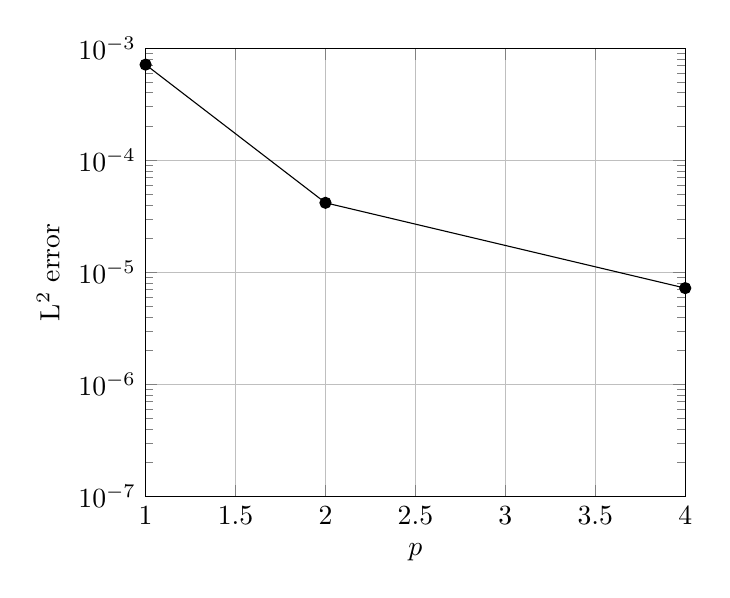
\begin{tikzpicture}
  \begin{axis}[
    %width=0.9\textwidth,
    %height=0.9\textwidth,
    grid=major,
    xlabel={$p$},
    ylabel={L$^2$ error},
  	%xmode=log,
  	ymode=log,
  	xmin=1,xmax=4,
  	ymin=1e-7,ymax=1e-3,
  	]
\addplot[mark=*, mark size=2, draw=black, mark options={solid, fill=black}] table[row sep=crcr] {
1 0.00071301712 \\
2 4.1717384e-05 \\
4 7.2301065e-06 \\};

  \end{axis}
\end{tikzpicture}
\caption{Accuracy of solutions for given angular quadrature using $S_8$ level-symmetric angular quadrature on a $2^\text{nd}$-order mesh with 120 zones.}
\label{fig:RZASMMSLinearRhoBrunnerS8g2r2Accuracy}
\end{figure}

\FloatBarrier

We investigated the symmetry preservation my performing sequential mesh refinements for $p=1$ with $S_8$ level-symmetric angular quadrature. Figures~\ref{fig:RZASMMSLinearRhoBrunnerp1S8g2Part1}~and~\ref{fig:RZASMMSLinearRhoBrunnerp1S8g2Part2} show the first several mesh refinement steps. The asymmetry is plotted on a log scale. The scale colors assist in demonstrating the qualitative locations of the asymmetries. The yellow region is the least symmetric, red regions have increased symmetry, and blue regions have the most symmetry. The $\phi_\text{sym}$ solution is plotted using the same finite element shape functions as the scalar flux. As on the $1^\text{st}$-order mesh, there is tremendous gain (many orders of magnitude) in symmetry by refining the $2^\text{nd}$-order mesh. We observe large regions of $\phi_\text{sym}$ changing from yellow to red to blue throughout the mesh refinement. Plotting the symmetry values as a function of the spherical radius (i.e., $\rho=\sqrt{r^2+z^2}$) in Figure~\ref{fig:RZASMMSLinearRhoBrunnerp1S8g2Nodes} confirms the substantial symmetry gain by refining the mesh. The largest asymmetry magnitude of the scalar flux remains near the origin (i.e. $\rho=\sqrt{r^2+z^2}=0$) as previously seen, but also remains prevalent in the discrete ordinates directions as though there were ray effects.

\begin{sidewaysfigure}[!htb]
\centering
\begin{subfigure}{0.33\textwidth}
\includegraphics[scale=0.3,trim={50pt 70pt 320pt 45pt},clip]{../../Research/graphics/Axisymmetry/RZASMMSLinearRhoBrunner/p1S8g2r0CompR}
\caption{$N_\text{zones}=6$.}
\end{subfigure}%
\begin{subfigure}{0.33\textwidth}
\includegraphics[scale=0.3,trim={50pt 70pt 320pt 45pt},clip]{../../Research/graphics/Axisymmetry/RZASMMSLinearRhoBrunner/p1S8g2r1CompR}
\caption{$N_\text{zones}=28$.}
\end{subfigure}%
\begin{subfigure}{0.33\textwidth}
\includegraphics[scale=0.3,trim={50pt 70pt 320pt 45pt},clip]{../../Research/graphics/Axisymmetry/RZASMMSLinearRhoBrunner/p1S8g2r2CompR}
\caption{$N_\text{zones}=120$.}
\end{subfigure}
\caption{Relative asymmetry for $p=1$ finite elements on a $2^\text{nd}$-order mesh for $S_8$ level-symmetric angular quadrature.}
\label{fig:RZASMMSLinearRhoBrunnerp1S8g2Part1}
\end{sidewaysfigure}

\begin{sidewaysfigure}[!htb]
\centering
\begin{subfigure}{0.33\textwidth}
\includegraphics[scale=0.3,trim={50pt 70pt 320pt 45pt},clip]{../../Research/graphics/Axisymmetry/RZASMMSLinearRhoBrunner/p1S8g2r3CompR}
\caption{$N_\text{zones}=496$.}
\end{subfigure}%
\begin{subfigure}{0.33\textwidth}
\includegraphics[scale=0.3,trim={50pt 70pt 320pt 45pt},clip]{../../Research/graphics/Axisymmetry/RZASMMSLinearRhoBrunner/p1S8g2r4CompR}
\caption{$N_\text{zones}=2016$.}
\end{subfigure}%
\begin{subfigure}{0.33\textwidth}
\includegraphics[scale=0.3,trim={50pt 70pt 320pt 45pt},clip]{../../Research/graphics/Axisymmetry/RZASMMSLinearRhoBrunner/p1S8g2r5CompR}
\caption{$N_\text{zones}=8128$.}
\end{subfigure}
\caption{Relative asymmetry for $p=1$ finite elements on a $2^\text{nd}$-order mesh for $S_8$ level-symmetric angular quadrature; mesh overlay may be removed for clarity.}
\label{fig:RZASMMSLinearRhoBrunnerp1S8g2Part2}
\end{sidewaysfigure}

\begin{figure}[!htb]
\centering
\includegraphics[scale=1]{./graphics/RZASMMSLinearRhoBrunnerp1S8g2}
\caption{Measure of the asymmetry for each finite element node for $1^\text{st}$-order finite elements using $S_8$ level-symmetric angular quadrature on a $2^\text{nd}$-order mesh with various number of zones (see Figures~\ref{fig:RZASMMSLinearRhoBrunnerp1S8g2Part1}-\ref{fig:RZASMMSLinearRhoBrunnerp1S8g2Part2}).}
\label{fig:RZASMMSLinearRhoBrunnerp1S8g2Nodes}
\end{figure}

\begin{table}[!htb]
\centering
{\renewcommand{\arraystretch}{1.5}
\begin{tabular}{|c|c|}
\hline
$N_\text{unknowns}$ & L$^2$ error \\\hline
6 & 0.025725225 \\\hline
28 & 0.0025077394 \\\hline
120 & 0.00071301712 \\\hline
496 & 0.00023746835 \\\hline
2016 & 7.3058318e-05 \\\hline
8128 & 2.080903e-05 \\\hline
\end{tabular}}
\end{table}

\begin{figure}[!htb]
\centering
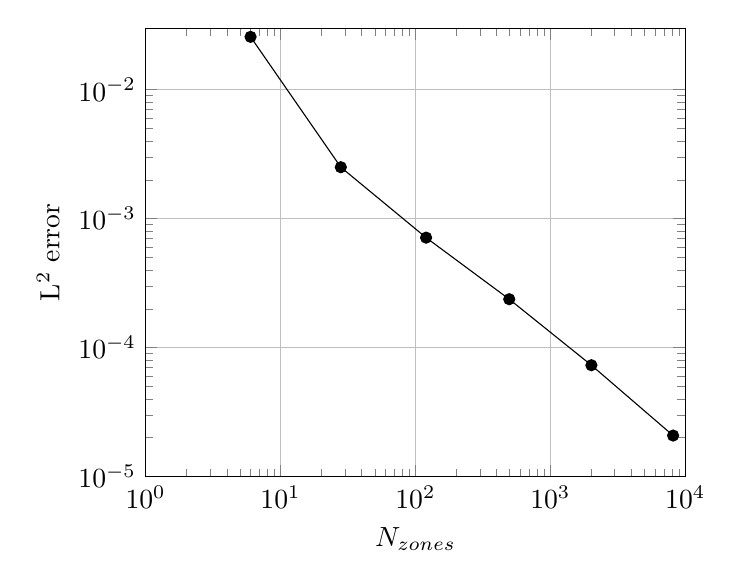
\begin{tikzpicture}
  \begin{axis}[
    %width=0.9\textwidth,
    %height=0.9\textwidth,
    grid=major,
    xlabel={$N_\text{zones}$},
    ylabel={L$^2$ error},
  	xmode=log,
  	ymode=log,
  	xmin=1,xmax=1e4,
  	ymin=1e-5,ymax=3e-2,
  	]
\addplot[mark=*, mark size=2, draw=black, mark options={solid, fill=black}] table[row sep=crcr] {
6 0.025725225 \\
28 0.0025077394 \\
120 0.00071301712 \\
496 0.00023746835 \\
2016 7.3058318e-05 \\
8128 2.080903e-05 \\};

  \end{axis}
\end{tikzpicture}
\caption{Accuracy of solutions for mesh refinement study using $p=1$, $S_8$ level-symmetric angular quadrature, on a $2^\text{nd}$-order mesh.}
\label{fig:RZASMMSLinearRhoBrunnerp1S8g2Accuracy}
\end{figure}

\FloatBarrier

We also investigated the symmetry preservation my performing sequential mesh refinements for $p=1$ with $S_8$ level-symmetric angular quadrature. Figures~\ref{fig:RZASMMSLinearRhoBrunnerp4S8g2Part1}~and~\ref{fig:RZASMMSLinearRhoBrunnerp4S8g2Part2} show the first several mesh refinement steps. The asymmetry is plotted on a log scale. The scale colors assist in demonstrating the qualitative locations of the asymmetries. The yellow region is the least symmetric, red regions have increased symmetry, and blue regions have the most symmetry. The $\phi_\text{sym}$ solution is plotted using the same finite element shape functions as the scalar flux. As on the $1^\text{st}$-order mesh, there is tremendous gain (many orders of magnitude) in symmetry by refining the $2^\text{nd}$-order mesh. We observe large regions of $\phi_\text{sym}$ changing from yellow to red to blue throughout the mesh refinement. Plotting the symmetry values as a function of the spherical radius (i.e., $\rho=\sqrt{r^2+z^2}$) in Figure~\ref{fig:RZASMMSLinearRhoBrunnerp4S8g2Nodes} confirms the substantial symmetry gain by refining the mesh. The largest asymmetry magnitude of the scalar flux remains near the origin (i.e. $\rho=\sqrt{r^2+z^2}=0$) as previously seen, but also remains prevalent in the discrete ordinates directions as though there were ray effects.

\begin{sidewaysfigure}[!htb]
\centering
\begin{subfigure}{0.33\textwidth}
\includegraphics[scale=0.3,trim={50pt 70pt 320pt 45pt},clip]{../../Research/graphics/Axisymmetry/RZASMMSLinearRhoBrunner/p4S8g2r0CompR}
\caption{$N_\text{zones}=6$.}
\end{subfigure}%
\begin{subfigure}{0.33\textwidth}
\includegraphics[scale=0.3,trim={50pt 70pt 320pt 45pt},clip]{../../Research/graphics/Axisymmetry/RZASMMSLinearRhoBrunner/p4S8g2r1CompR}
\caption{$N_\text{zones}=28$.}
\end{subfigure}%
\begin{subfigure}{0.33\textwidth}
\includegraphics[scale=0.3,trim={50pt 70pt 320pt 45pt},clip]{../../Research/graphics/Axisymmetry/RZASMMSLinearRhoBrunner/p4S8g2r2CompR}
\caption{$N_\text{zones}=120$.}
\end{subfigure}
\caption{Relative asymmetry for $p=4$ finite elements on a $2^\text{nd}$-order mesh for $S_8$ level-symmetric angular quadrature.}
\label{fig:RZASMMSLinearRhoBrunnerp4S8g2Part1}
\end{sidewaysfigure}

\begin{sidewaysfigure}[!htb]
\centering
\begin{subfigure}{0.33\textwidth}
\includegraphics[scale=0.3,trim={50pt 70pt 320pt 45pt},clip]{../../Research/graphics/Axisymmetry/RZASMMSLinearRhoBrunner/p4S8g2r3CompR}
\caption{$N_\text{zones}=496$.}
\end{subfigure}%
\begin{subfigure}{0.33\textwidth}
\includegraphics[scale=0.3,trim={50pt 70pt 320pt 45pt},clip]{../../Research/graphics/Axisymmetry/RZASMMSLinearRhoBrunner/p4S8g2r4CompR}
\caption{$N_\text{zones}=2016$.}
\end{subfigure}%
\begin{subfigure}{0.33\textwidth}
\includegraphics[scale=0.3,trim={50pt 70pt 320pt 45pt},clip]{../../Research/graphics/Axisymmetry/RZASMMSLinearRhoBrunner/p4S8g2r5CompR}
\caption{$N_\text{zones}=8128$.}
\end{subfigure}
\caption{Relative asymmetry for $p=4$ finite elements on a $2^\text{nd}$-order mesh for $S_8$ level-symmetric angular quadrature; mesh overlay may be removed for clarity.}
\label{fig:RZASMMSLinearRhoBrunnerp4S8g2Part2}
\end{sidewaysfigure}

\begin{figure}[!htb]
\centering
\includegraphics[scale=1]{./graphics/RZASMMSLinearRhoBrunnerp4S8g2.pdf}
\caption{Measure of the asymmetry for each finite element node for $4^\text{th}$-order DFEM, $S_8$ level-symmetric angular quadrature, and $2^\text{nd}$-order mesh with various number of zones (see Figures~\ref{fig:RZASMMSLinearRhoBrunnerp4S8g2Part1}~-~\ref{fig:RZASMMSLinearRhoBrunnerp4S8g2Part2}).}
\label{fig:RZASMMSLinearRhoBrunnerp4S8g2Nodes}
\end{figure}

\begin{table}[!htb]
\centering
{\renewcommand{\arraystretch}{1.5}
\begin{tabular}{|c|c|}
\hline
$N_\text{zones}$ & L$^2$ error \\\hline
6 & 0.0023130263 \\\hline
28 & 0.00010926868 \\\hline
120 & 7.2301065e-06 \\\hline
496 & 5.3684571e-07 \\\hline
2016 & 3.9184195e-08 \\\hline
8128 & 2.714164e-09 \\\hline
\end{tabular}}
\end{table}

\begin{figure}[!htb]
\centering
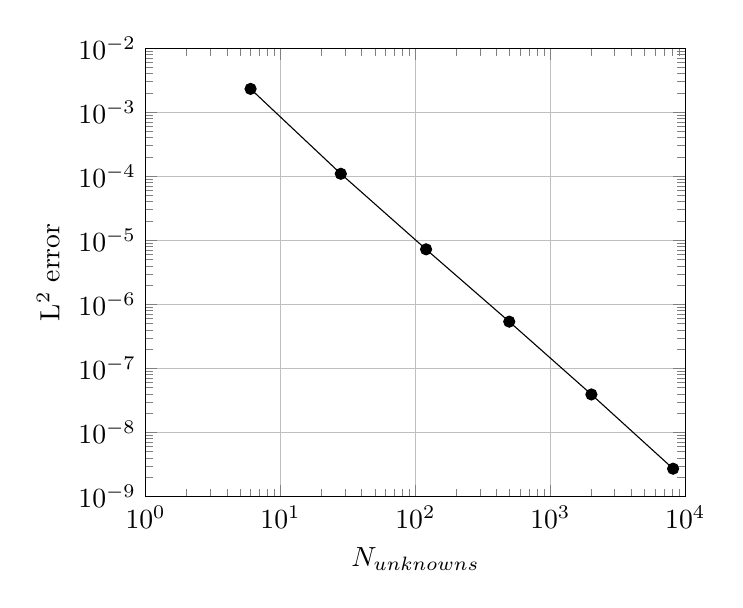
\begin{tikzpicture}
  \begin{axis}[
    %width=0.9\textwidth,
    %height=0.9\textwidth,
    grid=major,
    xlabel={$N_\text{unknowns}$},
    ylabel={L$^2$ error},
  	xmode=log,
  	ymode=log,
  	xmin=1,xmax=1e4,
  	ymin=1e-9,ymax=1e-2,
  	]
\addplot[mark=*, mark size=2, draw=black, mark options={solid, fill=black}] table[row sep=crcr] {
6 0.0023130263 \\
28 0.00010926868 \\
120 7.2301065e-06 \\
496 5.3684571e-07 \\
2016 3.9184195e-08 \\
8128 2.714164e-09 \\};

  \end{axis}
\end{tikzpicture}
\caption{Accuracy of solutions for mesh refinement study using $p=4$, $S_8$ level-symmetric angular quadrature, on a $2^\text{nd}$-order mesh.}
\label{fig:RZASMMSLinearRhoBrunnerp4S8g2Accuracy}
\end{figure}

\FloatBarrier

In the most refined case of Figures~\ref{fig:RZASMMSLinearRhoBrunnerp1S8g2Part2}~and~\ref{fig:RZASMMSLinearRhoBrunnerp4S8g2Par2}, we observe some ray effects. These effects are dependent on the discrete ordinates discretization order. Here, we investigate the symmetry preservation by performing sequential discrete ordinates refinements for $p=1$ on a $2^\text{nd}$-order mesh with 8128 zones. Figure~\ref{fig:RZASMMSLinearRhoBrunnerp1g2r5} show the first several mesh refinement steps. The asymmetry is plotted on a log scale. The scale colors assist in demonstrating the qualitative locations of the asymmetries. The yellow region is the least symmetric, red regions have increased symmetry, and blue regions have the most symmetry. The $\phi_\text{sym}$ solution is plotted using the same finite element shape functions as the scalar flux. The ray effects are dependent upon the discrete ordinates discretization order. Despite the appearance of a reduction in overall symmetry, plotting the symmetry values as a function of the spherical radius (i.e., $\rho=\sqrt{r^2+z^2}$) in Figure~\ref{fig:RZASMMSLinearRhoBrunnerp4S8g2Nodes} demonstrates that the overall asymmetry is not very dependent upon the discrete ordinates discretization. The locations of these ray effects may introduce asymmetries themselves when coupling to other phsyics.

\begin{sidewaysfigure}[!htb]
\centering
\begin{subfigure}{0.33\textwidth}
\includegraphics[scale=0.3,trim={50pt 70pt 320pt 45pt},clip]{../../Research/graphics/Axisymmetry/RZASMMSLinearRhoBrunner/p1S4g2r5}
\caption{$S_4$.}
\end{subfigure}%
%\begin{subfigure}{0.2\textwidth}
%\includegraphics[scale=0.25,trim={50pt 70pt 320pt 45pt},clip]{../../Research/graphics/Axisymmetry/RZASMMSLinearRhoBrunner/p1S6g2r5}
%\caption{$S_6$.}
%\end{subfigure}%
\begin{subfigure}{0.33\textwidth}
\includegraphics[scale=0.3,trim={50pt 70pt 320pt 45pt},clip]{../../Research/graphics/Axisymmetry/RZASMMSLinearRhoBrunner/p1S8g2r5-2}
\caption{$S_8$ (repeated from Fig.~\ref{fig:RZASMMSLinearRhoBrunnerp1S8g2Part2}).}
\end{subfigure}%
%\begin{subfigure}{0.2\textwidth}
%\includegraphics[scale=0.25,trim={50pt 70pt 320pt 45pt},clip]{../../Research/graphics/Axisymmetry/RZASMMSLinearRhoBrunner/p1S10g2r5}
%\caption{$S_{10}$.}
%\end{subfigure}%
\begin{subfigure}{0.33\textwidth}
\includegraphics[scale=0.3,trim={50pt 70pt 320pt 45pt},clip]{../../Research/graphics/Axisymmetry/RZASMMSLinearRhoBrunner/p1S12g2r5}
\caption{$S_{12}$.}
\end{subfigure}
\caption{Relative asymmetry for $p=1$ finite elements on a $2^\text{nd}$-order mesh with 8128 zones; mesh overlay may be removed for clarity.}
\label{fig:RZASMMSLinearRhoBrunnerp1g2r5}
\end{sidewaysfigure}

We also plot the asymmetry values as a function of the spherical radius (i.e., $\rho=\sqrt{r^2+z^2}$). Figure~\ref{fig:RZASMMSLinearRhoBrunnerp1g2r5Nodes} shows the $\phi_\text{sym}$ values calculated using Equation~\ref{eq:RelativeAsymmetry} for $1^\text{st}$-order finite elements on a $2^\text{nd}$-order mesh with 8128 zones for several angular quadrature discretizations.

\begin{figure}[!htb]
\centering
\includegraphics[scale=1]{./graphics/RZASMMSLinearRhoBrunnerp1g2r5.pdf}
\caption{Measure of the asymmetry for each finite element node for the given level-symmetric angular quadrature order for $1^\text{st}$-order DFEM and $2^\text{nd}$-order mesh with 8128 zones.}
\label{fig:RZASMMSLinearRhoBrunnerp1g2r5Nodes}
\end{figure}

\begin{table}[!htb]
\centering
{\renewcommand{\arraystretch}{1.5}
\begin{tabular}{|c|c|}
\hline
$S_N$ & L$^2$ error \\\hline
$S_4$ & 2.1057152e-05 \\\hline
$S_6$ & 2.0826499e-05 \\\hline
$S_8$ & 2.080903e-05 \\\hline
$S_{10}$ & 2.1015134e-05 \\\hline
$S_{12}$ & 2.1142207e-05 \\\hline
\end{tabular}}
\end{table}

\begin{figure}[!htb]
\centering
\begin{tikzpicture}
  \begin{axis}[
    %width=0.9\textwidth,
    %height=0.9\textwidth,
    grid=major,
    xlabel={$S_N$},
    ylabel={L$^2$ error},
  	%xmode=log,
  	ymode=log,
  	xmin=4,xmax=12,
  	ymin=1e-5,ymax=1e-4,
  	]
\addplot[mark=*, mark size=2, draw=black, mark options={solid, fill=black}] table[row sep=crcr] {
4 2.1057152e-05 \\
6 2.0826499e-05 \\
8 2.080903e-05 \\
10 2.1015134e-05 \\
12 2.1142207e-05 \\};

  \end{axis}
\end{tikzpicture}
\caption{Accuracy of solutions for given angular quadrature using $p=4$ on a $2^\text{nd}$-order mesh with 8128 zones.}
\label{fig:RZASMMSLinearRhoBrunnerp4g2r5Accuracy}
\end{figure}

\FloatBarrier

For completeness, we compare some of the nodal asymmetry plots for ease of comparing the $2^\text{nd}$-order mesh to the $1^\text{st}$-order mesh on the same scales.

\begin{figure}[!htb]
\centering
\begin{subfigure}{0.48\textwidth}
\centering
\includegraphics[width=\textwidth]{./graphics/RZASMMSLinearRhoBrunnerp1g1r2CompG.pdf}
\caption{$1^\text{st}$-order mesh (adapted from Figure~\ref{fig:RZASMMSLinearRhoBrunnerp1g1r2Nodes}).}
\end{subfigure}%
\hspace{0.04\textwidth}%
\begin{subfigure}{0.48\textwidth}
\centering
\includegraphics[width=\textwidth]{./graphics/RZASMMSLinearRhoBrunnerp1g2r2CompG.pdf}
\caption{$2^\text{nd}$-order mesh (adapted from Figure~\ref{fig:RZASMMSLinearRhoBrunnerp1g2r2Nodes}).}
\end{subfigure}
\caption{Measure of the asymmetry for each finite element node for the given level-symmetric angular quadrature order for $1^\text{st}$-order DFEM on the given mesh with 120 zones.}
\end{figure}

\begin{figure}[!htb]
\centering
\begin{subfigure}{0.48\textwidth}
\centering
\includegraphics[width=\textwidth]{./graphics/RZASMMSLinearRhoBrunnerp4g1r2CompG.pdf}
\caption{$1^\text{st}$-order mesh (adapted from Figure~\ref{fig:RZASMMSLinearRhoBrunnerp4g1r2Nodes}).}
\end{subfigure}%
\hspace{0.04\textwidth}%
\begin{subfigure}{0.48\textwidth}
\centering
\includegraphics[width=\textwidth]{./graphics/RZASMMSLinearRhoBrunnerp4g2r2CompG.pdf}
\caption{$2^\text{nd}$-order mesh (adapted from Figure~\ref{fig:RZASMMSLinearRhoBrunnerp4g2r2Nodes}).}
\end{subfigure}
\caption{Measure of the asymmetry for each finite element node for the given level-symmetric angular quadrature order for $4^\text{th}$-order DFEM on the given mesh with 120 zones.}
\end{figure}

\begin{figure}[!htb]
\centering
\begin{subfigure}{0.48\textwidth}
\centering
\includegraphics[width=\textwidth]{./graphics/RZASMMSLinearRhoBrunnerp4S8g1CompG.pdf}
\caption{$1^\text{st}$-order mesh (adapted from Figure~\ref{fig:RZASMMSLinearRhoBrunnerp4S8g1Nodes}).}
\end{subfigure}%
\hspace{0.04\textwidth}%
\begin{subfigure}{0.48\textwidth}
\centering
\includegraphics[width=\textwidth]{./graphics/RZASMMSLinearRhoBrunnerp4S8g2CompG.pdf}
\caption{$2^\text{nd}$-order mesh (adapted from Figure~\ref{fig:RZASMMSLinearRhoBrunnerp4S8g2Nodes}).}
\end{subfigure}
\caption{Measure of the asymmetry for each finite element node for $4^\text{th}$-order DFEM, $S_8$ level-symmetric angular quadrature, on the given mesh with various number of zones.}
\end{figure}

\FloatBarrier

%%%%%%%%%%%%%%%%%%%%%%%%%%%%%%%%%%%%%%%
\subsubsection{Axisymmety Summary and Discussion}
Table~\ref{tab:AxisymmetrySummary} summarizes our findings of whether or not each discretization property reduces the asymmetry or not.

\begin{table}[!htb]
\begin{tabular}{|c|c|}
\hline
Property & Reduce Asymmetry? \\\hline
$S_N$ order & no \\\hline
Finite element order & yes \\\hline
mesh refinement & yes \\\hline
mesh curvature & conditional \\\hline
\end{tabular}
\caption{Summary of discretizations and determination of whether they reduce the asymmetry.}
\label{tab:AxisymmetrySummary}
\end{table}

We observe that the asymmetry reduction stalled during mesh refinement for the low-order mesh (Figure~\ref{fig:RZASMMSLinearRhoBrunnerp4S8g1Nodes}. This was not the case for the high-order mesh (Figure~\ref{fig:RZASMMSLinearRhoBrunnerp1S8g2}. Since these were both calculated using $4^\text{th}$-order finite elements, the nodal scalar flux solutions at each spherical radius $\rho=\sqrt{r^2+z^2}$ are different.


Although the manufactured solution (Eq.~\ref{eq:RZMMSLinearRho}) is not overly complicated, a steep gradient appears in the MMS source term near $(r,z)=(0,0)$. We look at each term of the transport equation using the manufactured solution in Figure~\ref{fig:RZMMSLinearRhoAnalytic}. The shape of the source term $S_0/(2 \pi)$ is complicated near the origin. In practice, the source term is approximated by the finite element shape function using the analytic values for the nodes. So although the source is exact at the node points, the shape function does not capture the analytic shape of the source term necessary to achieve the axisymmetry we desire.

We note that this mesh is made up entirely of quadrilaterals, even the inner-most radial zones.

\begin{figure}
\includegraphics[scale=0.5]{../../Research/graphics/Axisymmetry/RZASMMSLinearRho/TransportTerms}
\caption{Analytic representation of each term of the transport equation using the manufactured solution, Equation~\ref{eq:RZMMSLinearRho}, for $(\mu,\xi)=(0.21821789023599239,0.95118973121134187)$. The complicated shapes of the streaming and source terms are typical of the other $\vec{\Omega}$ directions.}
\label{fig:RZMMSLinearRhoAnalytic}
\end{figure}

\FloatBarrier

%%%%%%%%%%%%%%%%%%%%%%%%%%%%%%%%%%%%%%%
\subsection{Strong Scatter with Alternating Boundaries Test}
\label{sec:StrongScatter}
We previously tested our higher-order \XY\ transport methodology on an optically thick and highly scattering problem~\cite{WoodsHoDgfemXyCurved}. Here, we perform the same calculation in \RZ\ geometry as originally introduced by Palmer and Adams~\cite{PalmerCurvilinearTransport} and Palmer~
\cite{PalmerDissertation}. The medium is homogeneous, highly scattering ($c=0.999$), has cross sections $\sigma_t=1000 \text{ cm}^{-1}$, $\sigma_s = 999 \text{ cm}^{-1}$, and has no external source. The incident angular flux boundary conditions of strength $\psi_{inc} = 1/(2 \pi) \text{ cm}^{-1} \text{ s}^{-1}$ on alternating locations denoted in Figure~\ref{fig:StrongScatterProblem} by gray bars. This incident angular flux strength is an estimation to compare to previous research results~\cite{PalmerCurvilinearTransport,PalmerDissertation}. For comparison to previous research using BLD, we solve this problem using $p=1$ Gauss-Legendre DGFEM with $S_4$ level-symmetric angular quadrature. The solution is shown in Figure~\ref{fig:RZTP2S4e1}. We observe oscillations in the solution that result in some negative scalar fluxes. The solution changes about 12 orders of magnitude. Compared to other research~\cite{PalmerDissertation}, we observe similar oscillations in the boundary layers, however our solution also presents oscillations in the problem interior. This may be due to the use of different basis functions or a result of not discretizing the conservation equation (Eq.~\ref{eq:RZTransport}).

We also solve with $S_8$ level-symmetric angular quadrature using $4^\text{th}$-order finite elements. This solution is shown in Figure~\ref{fig:RZTP2S8e4}. We observe oscillations in the scalar flux that results in negative solutions. These are predominantly in the boundary layer regions near the upper right and lower left. The solution changes about 20 orders of magnitude.

\begin{figure}[!htb]
\centering
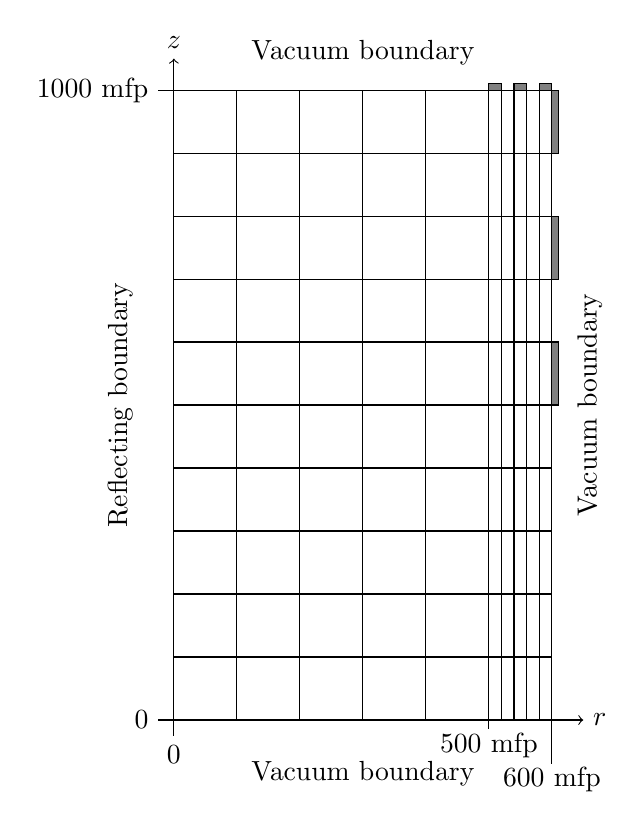
\begin{tikzpicture}[scale=0.8]
\draw [->] (0,0) -- (6.5,0);
\draw [->] (0,0) -- (0,10.5);
\node [above] at (0,10.5) {$z$};
\node [right] at (6.5,0) {$r$};
\draw (0,-0.25) -- (0,0) -- (-0.25,0);
\draw (5,0) -- (5,-0.15);
\draw (6,0) -- (6,-0.7);
\draw (0,10) -- (-0.25,10);
\node [below] at (0,-0.25) {0};
\node [left] at (-0.25,0) {0};
\node [below] at (5,-0.05) {500 mfp};
\node [below] at (6,-0.6) {600 mfp};
\node [left] at (-0.25,10) {1000 mfp};
\node [below] at (3,-0.5) {Vacuum boundary};
\node [above] at (3,10.25) {Vacuum boundary};
\node [right] at (6.25,5) {\rotatebox{90}{Vacuum boundary}};
\node [left] at (-0.5,5) {\rotatebox{90}{Reflecting boundary}};
\draw (5.2,0) -- (5.2,10);
\draw (5.4,0) -- (5.4,10);
\draw (5.6,0) -- (5.6,10);
\draw (5.8,0) -- (5.8,10);
\draw [fill=gray] (5,10) rectangle (5.2,10.1);
\draw [fill=gray] (5.4,10) rectangle (5.6,10.1);
\draw [fill=gray] (5.8,10) rectangle (6,10.1);
\draw [fill=gray] (6,9) rectangle (6.1,10);
\draw [fill=gray] (6,7) rectangle (6.1,8);
\draw [fill=gray] (6,5) rectangle (6.1,6);
\draw (0,0) grid (6,10);
\end{tikzpicture}
\caption{Strong scatter with discontinuous BCs with MIP DSA problem geometry; gray boundaries indicate incident boundary locations.}
\label{fig:StrongScatterProblem}
\end{figure}

Comparing Figures~\ref{fig:RZTP2S4e1} and \ref{fig:RZTP2S8e4}, we observe that the areas of negative solution in the problem interior is suppressed with the use of higher-order finite elements. We also observe that the higher-order FEM modeled a steeper gradient in the solution. The HO solution drove an additional 8 orders of magnitude further than the LO solution. While refining the mesh may help the LO method to model the steep gradient, the HO method was able to do so.

\begin{figure}[!htb]
\centering
\begin{subfigure}{0.45\textwidth}
\centering
\includegraphics[scale=0.25]{../../Research/graphics/RZTP2S4e1blue}
\captionof{figure}{Scalar flux.}
\label{fig:RZTP2S8e4blue}
\end{subfigure}%
\hspace{0.05\textwidth}
\begin{subfigure}{0.45\textwidth}
\centering
\includegraphics[scale=0.25]{../../Research/graphics/RZTP2S4e1logblue}
\caption{Log of scalar flux.}
\label{fig:RZTP2S8e4logblue}
\end{subfigure}
\caption{Solution to strong scatter with discontinuous boundary conditions with $p=1$ finite elements and $S_4$ level-symmetric angular quadrature. White regions indicate negative scalar fluxes.}
\label{fig:RZTP2S4e1}
\end{figure}

\begin{figure}[!htb]
\centering
\begin{subfigure}{0.45\textwidth}
\centering
\includegraphics[scale=0.25]{../../Research/graphics/RZTP2S8e4blue}
\captionof{figure}{Scalar flux.}
\label{fig:RZTP2S8e4blue}
\end{subfigure}%
\hspace{0.05\textwidth}
\begin{subfigure}{0.45\textwidth}
\centering
\includegraphics[scale=0.25]{../../Research/graphics/RZTP2S8e4logblue}
\caption{Log of scalar flux.}
\label{fig:RZTP2S8e4logblue}
\end{subfigure}
\caption{Solution to strong scatter with discontinuous boundary conditions with $p=4$ finite elements and $S_8$ level-symmetric angular quadrature. White regions indicate negative scalar fluxes.}
\label{fig:RZTP2S8e4}
\end{figure}

\begin{figure}[!htb]
\centering
\begin{subfigure}{0.45\textwidth}
\centering
\includegraphics[scale=0.25]{../../Research/graphics/TP2RZS12p4g2blue}
\captionof{figure}{Scalar flux.}
\label{fig:TP2RZS12p4g2blue}
\end{subfigure}%
\hspace{0.05\textwidth}
\begin{subfigure}{0.45\textwidth}
\centering
\includegraphics[scale=0.25]{../../Research/graphics/TP2RZS12p4g2logblue}
\caption{Log of scalar flux.}
\label{fig:TP2RZS12p4g2logblue}
\end{subfigure}
\caption{Solution to strong scatter with discontinuous boundary conditions with $p=4$ finite elements and $S_{12}$ level-symmetric angular quadrature on a $2^\text{nd}$-order mesh. White regions indicate negative scalar fluxes.}
\label{fig:TP2RZS12p4g2}
\end{figure}

%%%%%%%%%%%%%%%%%%%%%%%%%%%%%%%%%%%%%%%
\subsection{Material Discontinuity Stress Test}
We adapted this problem from Palmer \cite{PalmerDissertation} and solved it without DSA in Woods et al. \cite{WoodsHoDgfemXyCurved}. There are five different material regions described in Table \ref{tab:MaterialDiscontinuityProperties} and Figure \ref{fig:MaterialDiscontinuityMesh}.

\begin{table}[!htb]
\centering
{\renewcommand{\arraystretch}{1.5}
\begin{tabular}{|c|c|c|c|}
\hline
Material Region & $\sigma_t$ cm$^{-1}$ & $\sigma_s$ cm$^{-1}$ & $S_0 \text{ cm}^{-2} \text{ s}^{-1}$ \\\hline
Source & 1.0 & 1.0 & 1.0 \\
Very thin absorber & 0.0001 & 0.0 & 0.0 \\
Thick absorber & 10.0 & 0.0 & 0.0 \\
Very thick absorber & 100.0 & 0.0 & 0.0 \\
Very thick scatterer & 1000.0 & 1000.0 & 0.0 \\
\hline
\end{tabular}}
\caption{Material discontinuity stress test with MIP DSA material properties.}
\label{tab:MaterialDiscontinuityProperties}
\end{table}

\begin{figure}[!hp]
\centering
\begin{tikzpicture}[scale=0.8]
\node [below] at (0,-0.25) {0};
\node [left] at (-0.25,0) {0};
\node [left] at (-0.25,10) {$z = 1$ cm};
\node [below] at (10,-0.25) {$r = 1$ cm};
\node [below] at (5,-0.5) {Vacuum boundary};
\node [above] at (5,10.25) {Vacuum boundary};
\node [right] at (10.25,5) {\rotatebox{90}{Vacuum boundary}};
\node [left] at (-0.5,5) {\rotatebox{90}{Reflecting boundary}};
\draw [fill=gray] (0,0) rectangle (2,10);
\draw [pattern= north west lines] (2,0) rectangle (6,2);
\draw [pattern=crosshatch dots] (2,2) rectangle (4,10);
\draw [pattern=crosshatch] (6,0) rectangle (10,2);
\draw (0,0) grid (10,10);
\node [fill=white] at (1,5) {Source};
\node [align=center,fill=white] at (4,1) {Very thin\\absorber};
\node [align=center,fill=white] at (3,6) {Thick\\absorber};
\node [align=center,fill=white] at (8,1) {Very thick\\absorber};
\node [align=center,fill=white] at (7,6) {Very thick\\scatterer};
\end{tikzpicture}
\caption{Material discontinuity stress test with MIP DSA problem geometry; materials defined in Table \ref{tab:MaterialDiscontinuityProperties}.}
\label{fig:MaterialDiscontinuityMesh}
\end{figure}

This problem has opacities that range several orders of magnitude, resulting in strong material discontinuities. We also introduce anisotropic incident intensities into the scattering region by preferentially attenuating intensities that are not perpendicular to the thick absorber. We expect some degradation in the DSA in problems with strong material discontinuities \cite{WangDissertation}. We also expect boundary layers to form from the anisotropic incident intensities \cite{AdamsDFEMDiffLimit}. The solution is shown in Figure~\ref{fig:RZMultiMaterial}.

\begin{figure}[!htb]
\centering
\begin{subfigure}{0.8\textwidth}
\centering
\includegraphics[scale=0.3,trim={50pt 140pt 50pt 80pt},clip]{../../Research/graphics/TP3RZS4e2}
\captionof{figure}{Scalar flux.}
\label{fig:TP2RZS4e4}
\end{subfigure}
\begin{subfigure}{0.8\textwidth}
\centering
\includegraphics[scale=0.3,trim={50pt 140pt 50pt 80pt},clip]{../../Research/graphics/TP3RZS4e2log}
\caption{Log of scalar flux.}
\label{fig:TP2RZS4e4}
\end{subfigure}
\caption{Solution to multi-material stress test. White regions indicate negative scalar fluxes.}
\label{fig:RZMultiMaterial}
\end{figure}


{\color{red}
%%%%%%%%%%%%%%%%%%%%%%%%%%%%%%%%%%%%%%%
\subsection{Reflecting Boundary Conditions}

To incorporate reflecting boundary conditions, we will ``guess'' the incident angular fluxes, update them with outgoing angular fluxes from the previous iteration, and adapt a convergence criterion for those fluxes. Along the z-axis, the reflection for direction $\vec{\Omega} = (\mu, \eta, \xi)$ is $\vec{\Omega}_R = (-\mu, \eta, \xi)$.

%%%%%%%%%%%%%%%%%%%%%%%%%%%%%%%%%%%%%%%
\subsection{Reflecting Boundary Conditions}
{\color{red}This may not warrant an entire subsection.}

Reflecting boundaries are dependent upon the direction of the outgoing angular flux, $\vec{\Omega}_m$. The reflected incident direction is
\begin{flalign}
\vec{\Omega}^R & = \vec{\Omega}_m - 2 \left(\vec{\Omega}_m \vd \hat{n} \right) \hat{n}
\end{flalign}
%
where $\vec{\Omega}_m$ is the outgoing direction and $\hat{n}$ is the unit normal vector on the boundary (pointing outward). We apply a Dirichlet boundary condition for the angular flux in the reflected direction,
\begin{flalign}
\psi^b(\vec{r},\vec{\Omega}^R) & = \psi_m
\end{flalign}
}

%%%%%%%%%%%%%%%%%%%%%%%%%%%%%%%%%%%%%%%
\subsection{\RZ\ Geometry Conclusions}
\label{sec:RZConclusions}
We discretized the transport equation in \RZ\ geometry and performed several test problems to qualitatively and quantitatively assess the behavior of our high-order finite element spatial discretization method. Instead of performing the spatial discretization on the conservation form of the transport equation, we performed a product rule and pulled a radius variable out of the $r$-derivative term. This allowed us to easily extend our \XY\ geometry implementation in MFEM to \RZ\ geometry. We discretized the direction of travel using level-symmetric angular quadrature and used the method of Morel and Montry to sweep across each angular quadrature level to solve for the angular flux at each discrete ordinate. The source iteration method was employed, where we calculate the scalar flux from a weighted sum of the angular fluxes, use that scalar flux in the scattering source, and iterate on the scalar flux until it converges.

Our method was sufficiently able to solve a uniform infinite medium problem. We extended our analysis to a spatial convergence study using the method of manufactured solutions. Our chosen manufactured solution is smooth everywhere and resulted in the expected $O(p+1)$ spatial convergence rates, which was expected from other research.

Finally, we performed a study on preserving axisymmetry (i.e. 1-D spherical symmetry). An ideal method will be able to solve a 1-D spherical problem using a \RZ\ geometry discretization. We solved using the method of manufactured solutions and determined a measure of symmetry. We varied the finite element order, angular quadrature order, spatial refinement, and mesh order.
{\color{blue}For a $1^\text{st}$-order mesh...}

For a $2^\text{nd}$-order mesh, we determined that the angular quadrature order has very little impact on the relative symmetry of the solution. At a sufficient mesh refinement, the relative symmetry produces distinct ``rays''. The number of these rays increases with the angular quadrature order. However, these rays were drastically damped by increasing the finite element order.

In future work, we will investigate alternative methods for handling the angular derivative. Warsa and Prinja~\cite{WarsaAngularQuadrature} proposed a method by performing a product rule on the angular derivative. We will also implement the numerical solution to the conservative form of the radiation transport equation in \RZ\ geometry.

It is common for the solution to the thermal radiation transport equation to be averaged over each mesh zone to be used in the energy balance equation for hydrodynamics calculations. We will also consider cell average axisymmetry. Also for the axisymmetric manufactured solution, we would like to develop other manufactured solutions that have simpler manufactured source terms near the origin. The complicated source term that we used was sufficient for $(r,z)$ coordinates further from the origin, but the finite element approximated source term was not close enough to the analytical source near the origin to maintain symmetry. Lastly, the mesh used for the axisymmetry calculations was made entirely of quadrilaterals. That is, even the innermost zones were quadrilaterals with one vertex having a very oblique angle (nearly 180 degrees). We need to modify MFEM to handle mixed element types.



%\bibliographystyle{apalike}
%\bibliography{Thesis_bib}

\end{document}
